\chapter{小程序测试}

\section{登录功能测试}

功能描述:用户通过微信授权上传昵称和头像并登录到系统

用户操作:在“我的”页面下 点击授权登录

预期结果:后端返回请求数据(url、introduce、message、moblie、name、sex)服务器状态(result、message)字段信息.原“请授权登录”处显示用户的头像、昵称

测试结果:通过
\begin{figure}[htbp]
    \centering
    \begin{minipage}[t]{0.32\textwidth}
    \centering
    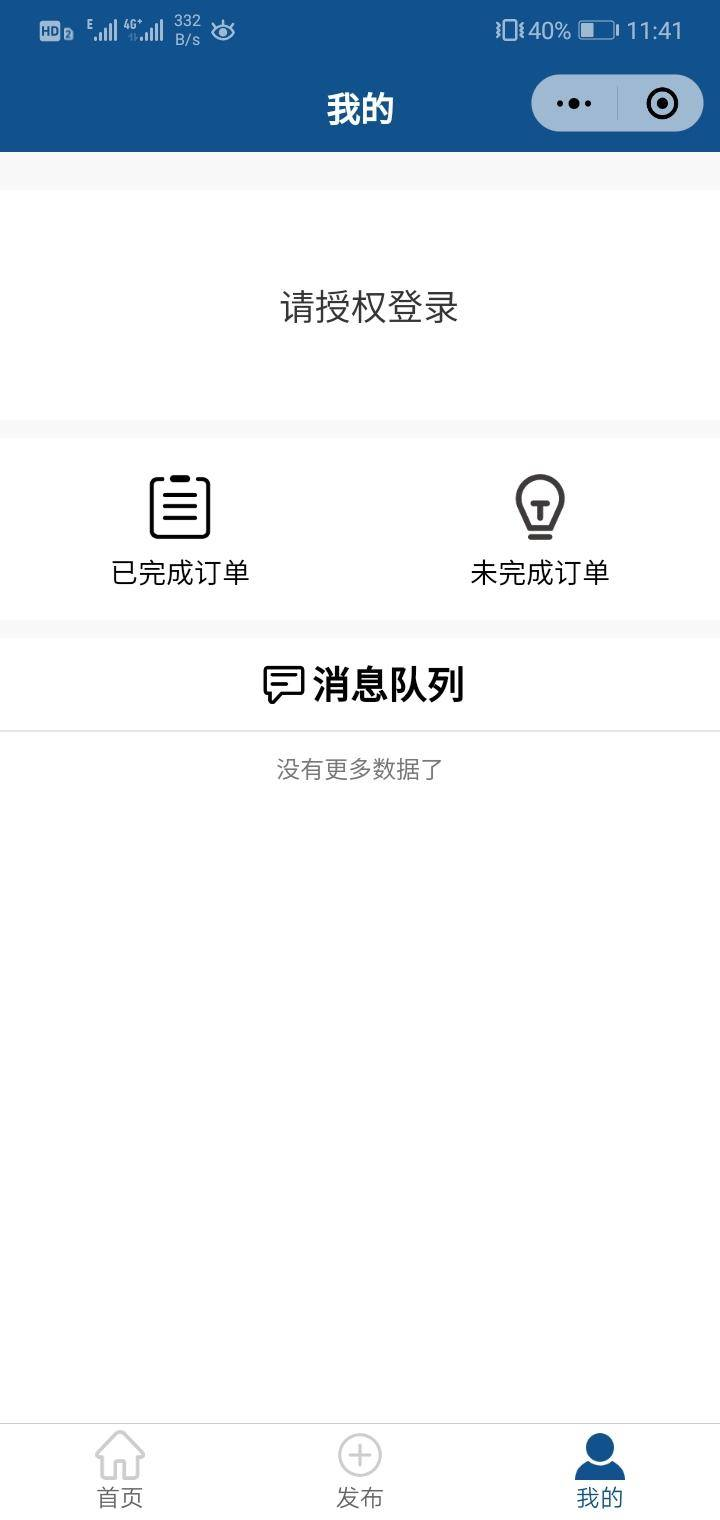
\includegraphics[width=3.8cm,height=8cm]{test/image/test1.png} 
    \caption{登录功能测试1}
    \end{minipage}
    \begin{minipage}[t]{0.32\textwidth}
    \centering
    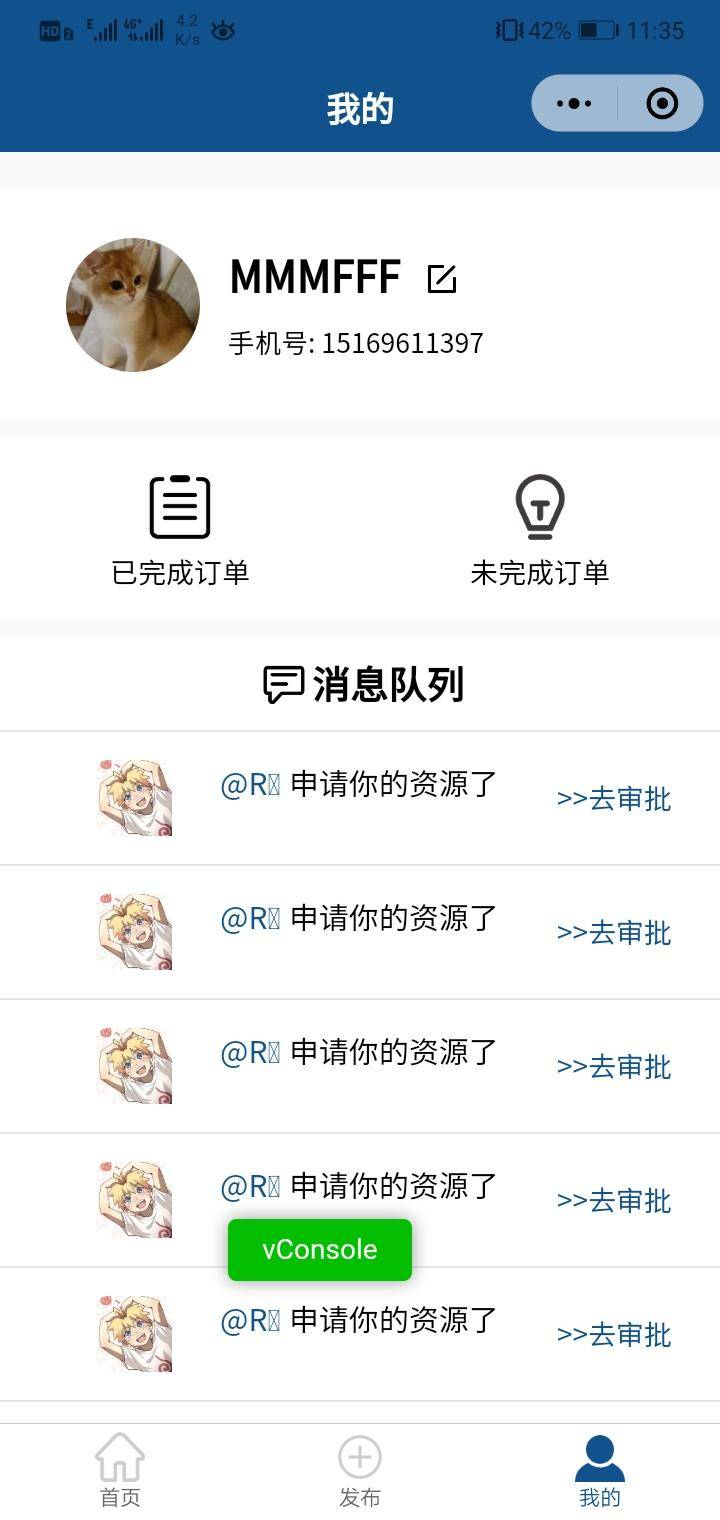
\includegraphics[width=3.8cm,height=8cm]{test/image/test2.png}
    \caption{登录功能测试2}
    \end{minipage}
    \begin{minipage}[t]{0.32\textwidth}
        \centering
        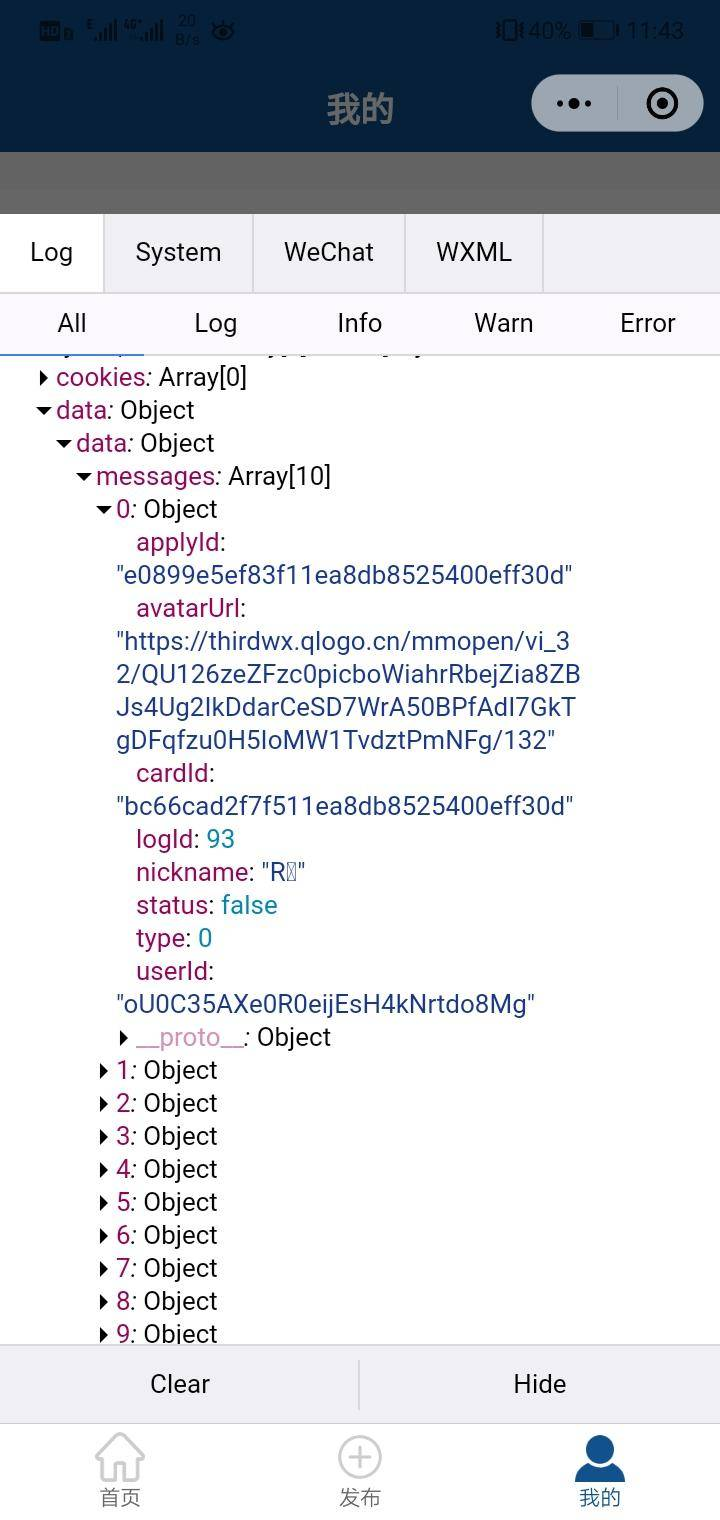
\includegraphics[width=3.8cm,height=8cm]{test/image/test3.png}
        \caption{测试结果}
        \end{minipage}
    \end{figure}

\section{通过手机号获取验证码功能测试}

功能描述:用户输入手机号,发送给服务器用于服务器发送验证码

用户操作:在“手机验证”界面下输入手机号点击获取验证码

预期结果:通过短信收到验证码,服务器返回状态码(result、message)

测试结果:通过

\newpage
\begin{figure}[htbp]
    \centering
    \begin{minipage}[t]{0.48\textwidth}
    \centering
    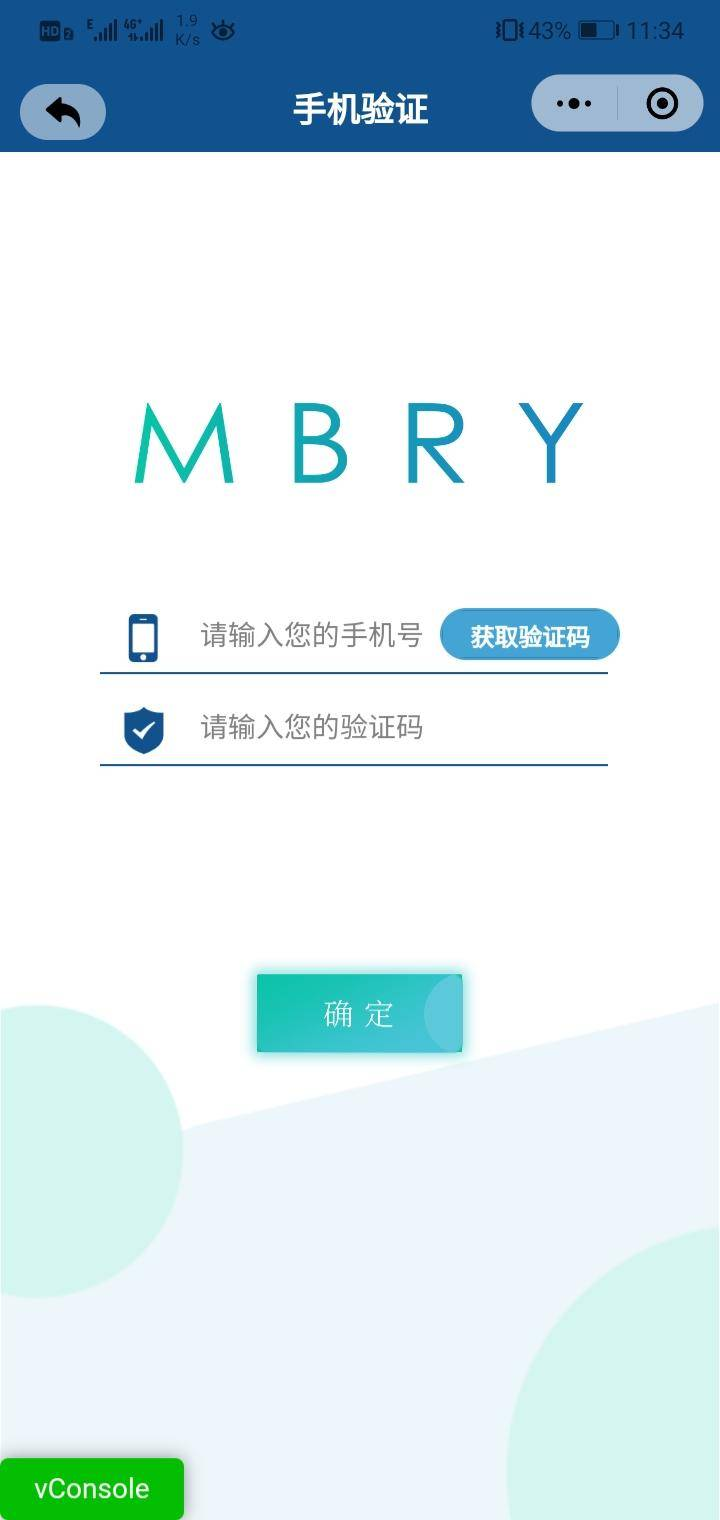
\includegraphics[width=4cm,height=8cm]{test/image/test4.png} 
    \caption{获取验证码}
    \end{minipage}
    \end{figure}
 
\section{绑定手机号功能测试}
功能描述:用户输入手机号验证码,绑定手机号

用户操作:在3.2基础上输入验证码

预期结果:页面跳转、提示绑定成功

测试结果:通过

\begin{figure}[htbp]
    \centering
    \begin{minipage}[t]{0.48\textwidth}
    \centering
    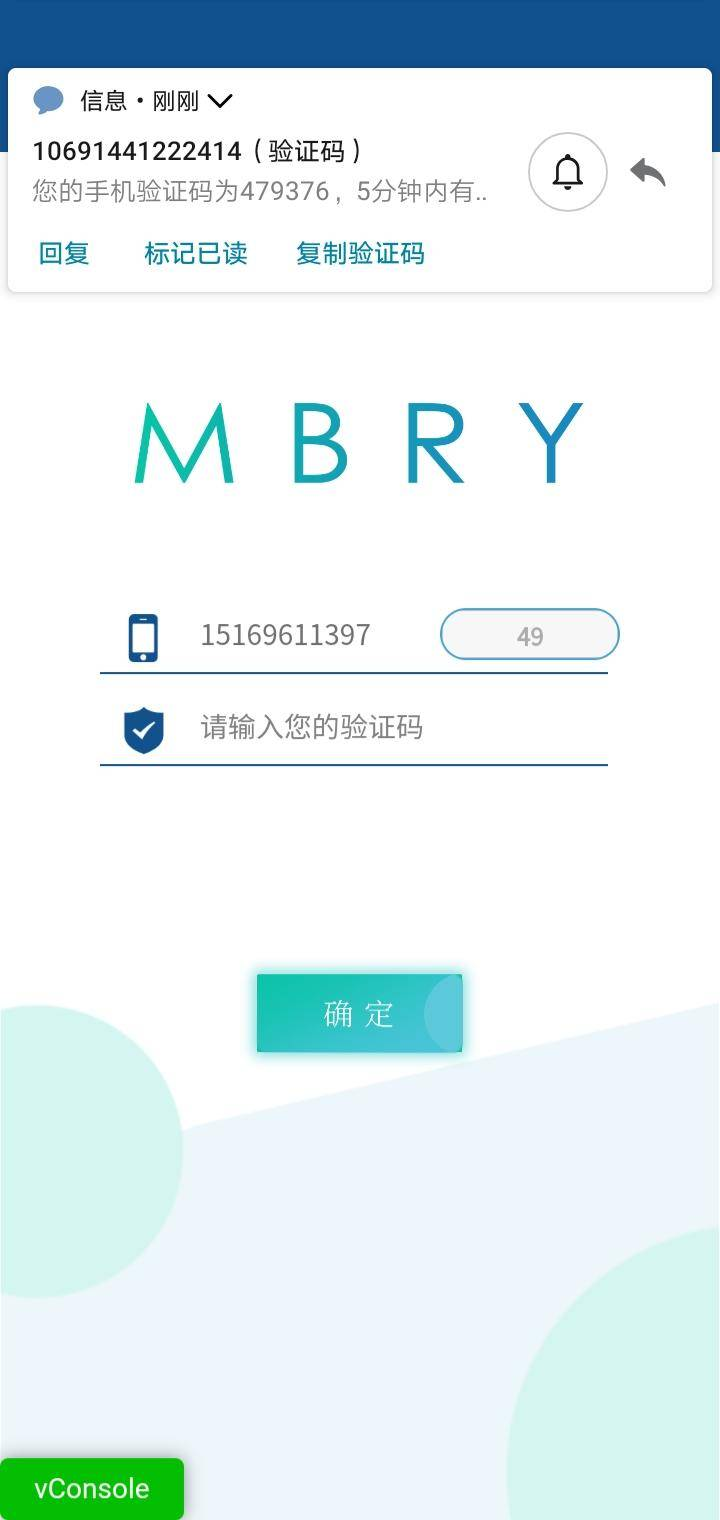
\includegraphics[width=4cm,height=8cm]{test/image/test5.png} 
    \caption{输入验证码}
    \end{minipage}
\end{figure}
\newpage

\section{浏览最新帖子功能测试}
实现用例1:房屋信息查询

功能描述:用户可在首页查看最新发布的帖子

用户操作:在“首页”页面下,用户可查看帖子列表。

预期结果:服务器返回帖子数据;在首页下半部分会按发布时间顺序展示最新发布的帖子,帖子列表可下拉

测试结果:通过

\begin{figure}[htbp]
    \centering
    \begin{minipage}[t]{0.48\textwidth}
    \centering
    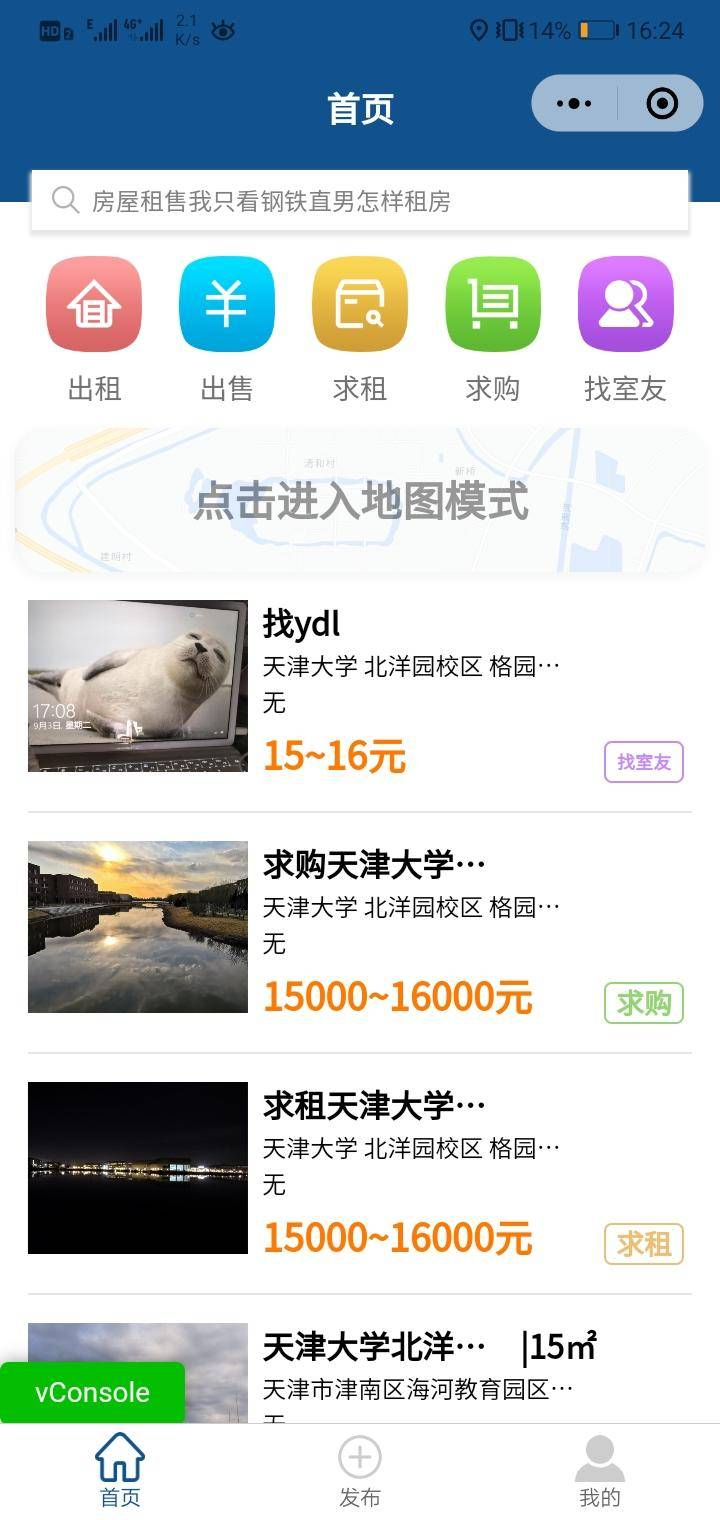
\includegraphics[width=4cm,height=8cm]{test/image/test6.png} 
    \caption{首页}
    \end{minipage}
    \begin{minipage}[t]{0.48\textwidth}
    \centering
    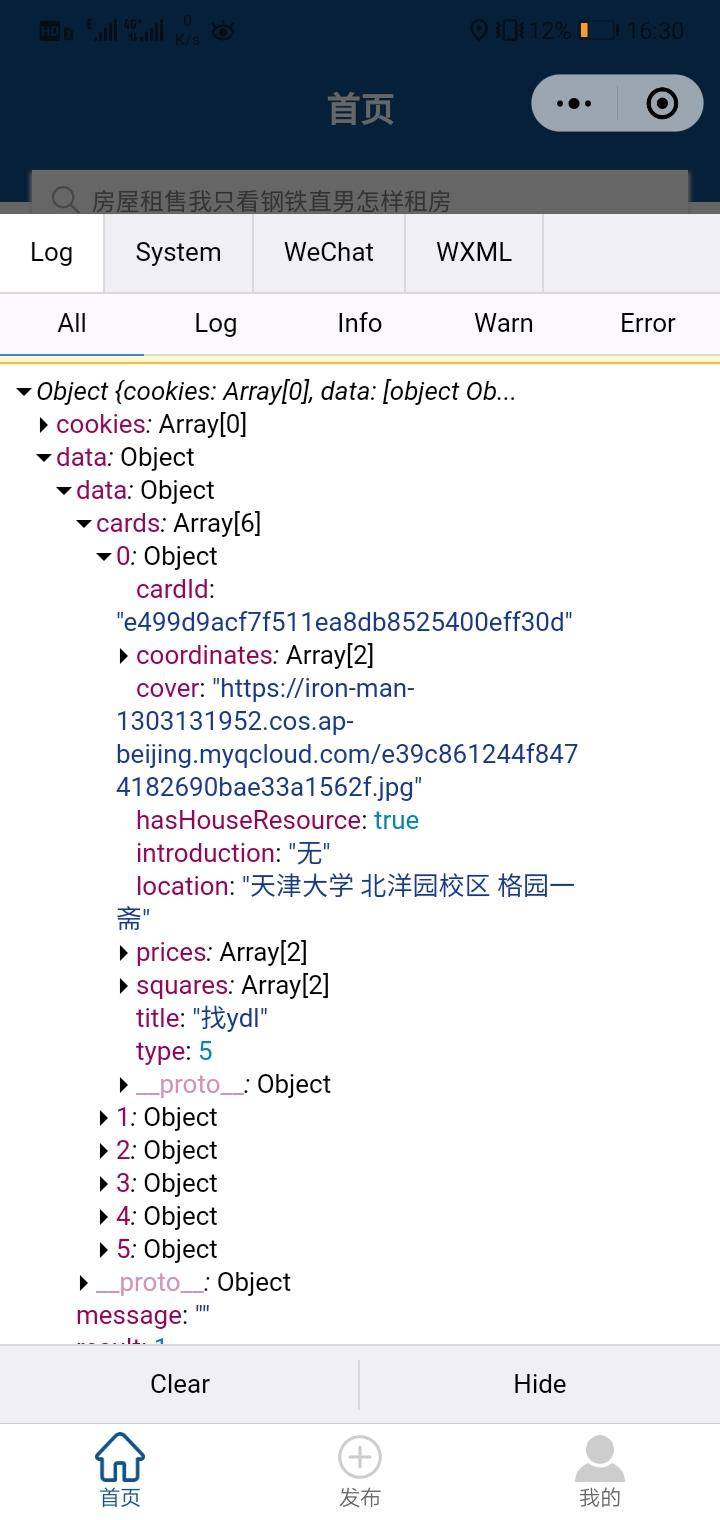
\includegraphics[width=4cm,height=8cm]{test/image/test7.png}
    \caption{测试结果}
    \end{minipage}
    \end{figure}
\section{查看出租帖子功能测试}
实现用例1:房屋信息查询

功能描述:用户可指定查看出租类型的帖子

用户操作:在“首页”页面下,点击出租 

预期结果:服务器返回出租帖子数据,进入出租帖子查询界面

测试结果:通过
\newpage

\begin{figure}[htbp]
    \centering
    \begin{minipage}[t]{0.32\textwidth}
        \centering
        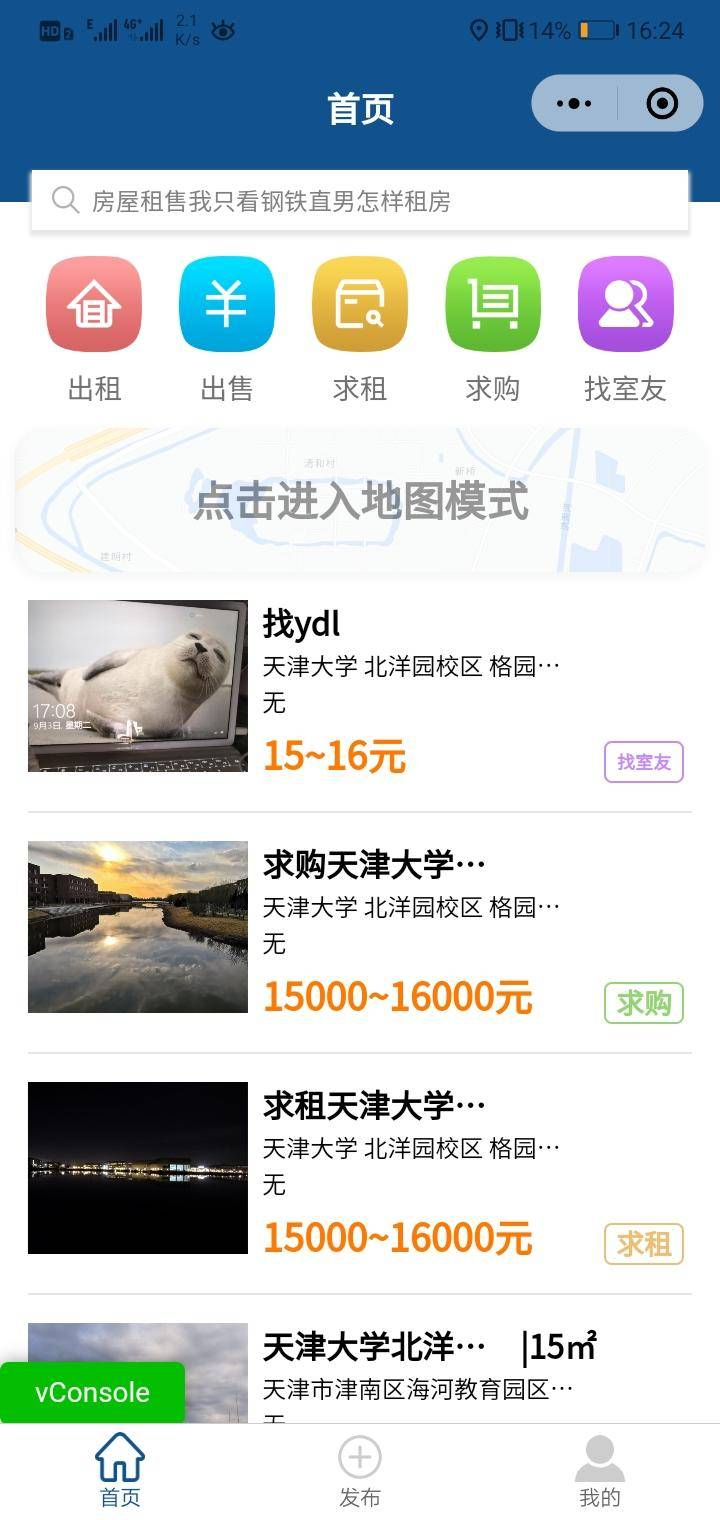
\includegraphics[width=3.8cm,height=8cm]{test/image/test8.png} 
       \caption{出租界面} 
        \end{minipage}
    \begin{minipage}[t]{0.32\textwidth}
    \centering
    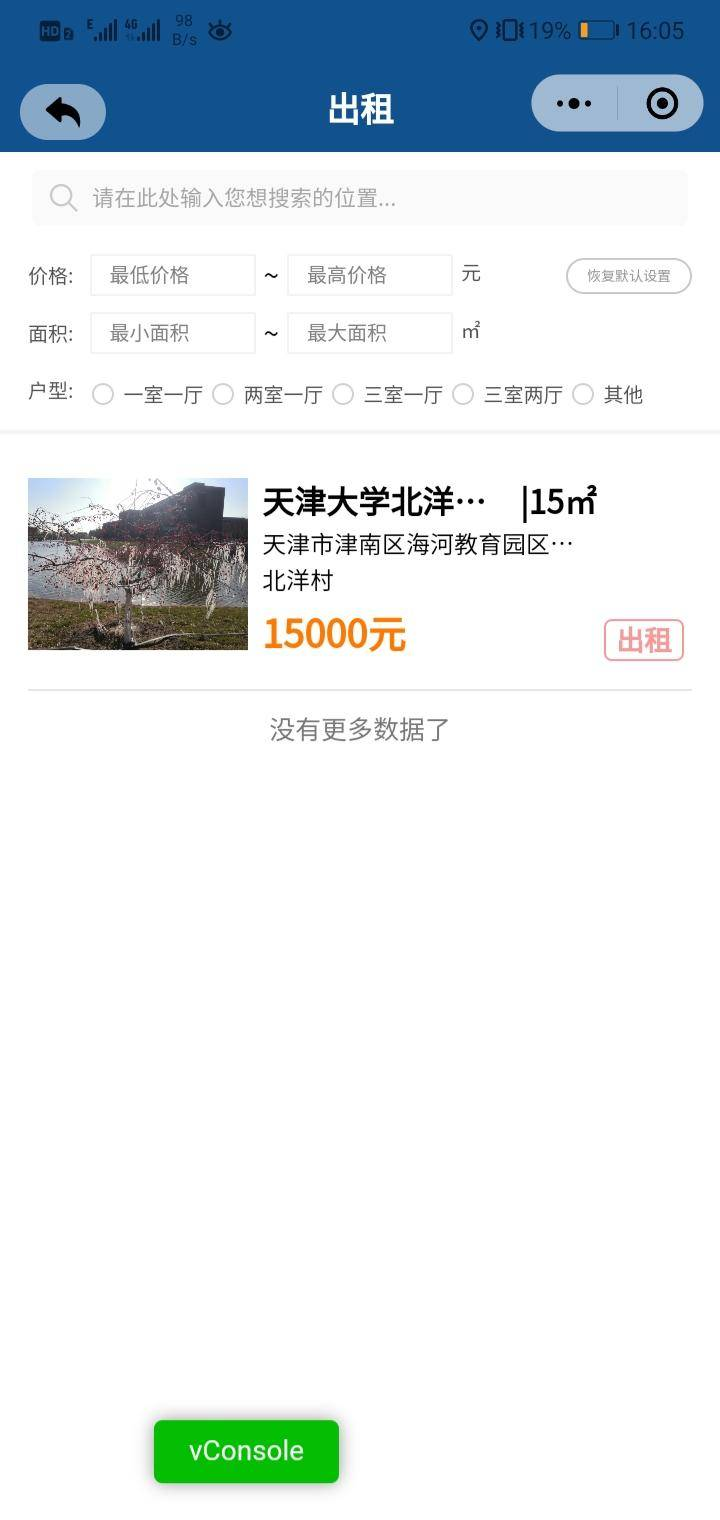
\includegraphics[width=3.8cm,height=8cm]{test/image/test9.png} 
   \caption{出租界面} 
    \end{minipage}
    \begin{minipage}[t]{0.32\textwidth}
    \centering
    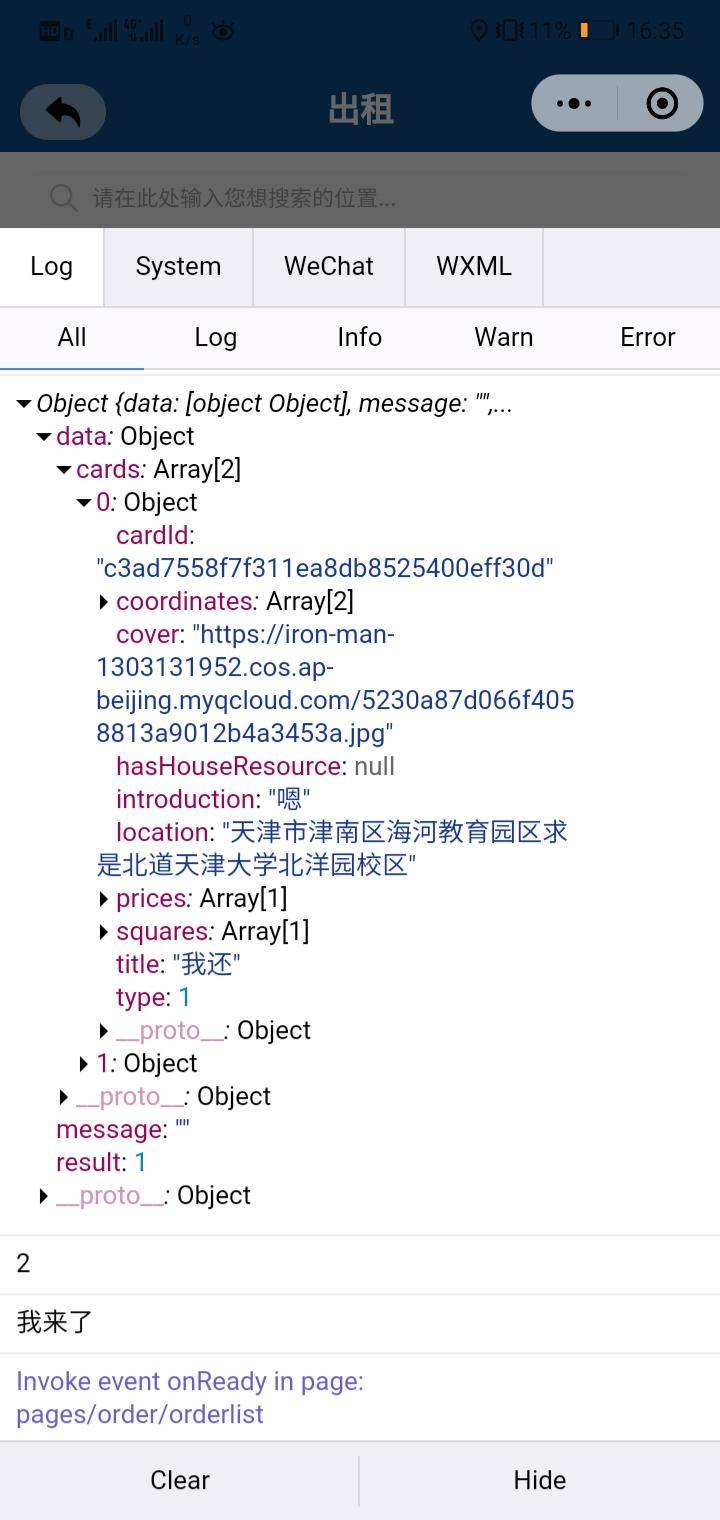
\includegraphics[width=3.8cm,height=8cm]{test/image/test10.png}
    \caption{测试结果}
    \end{minipage}
    \end{figure}

\section{查看出售帖子功能测试}
实现用例1:房屋信息查询

功能描述:用户可指定查看出售类型的帖子

用户操作:在“首页”页面下,点击出售

预期结果:服务器返回出售帖子数据,进入出售帖子查询界面

测试结果:通过

\begin{figure}[htbp]
    \centering
    \begin{minipage}[t]{0.32\textwidth}
        \centering
        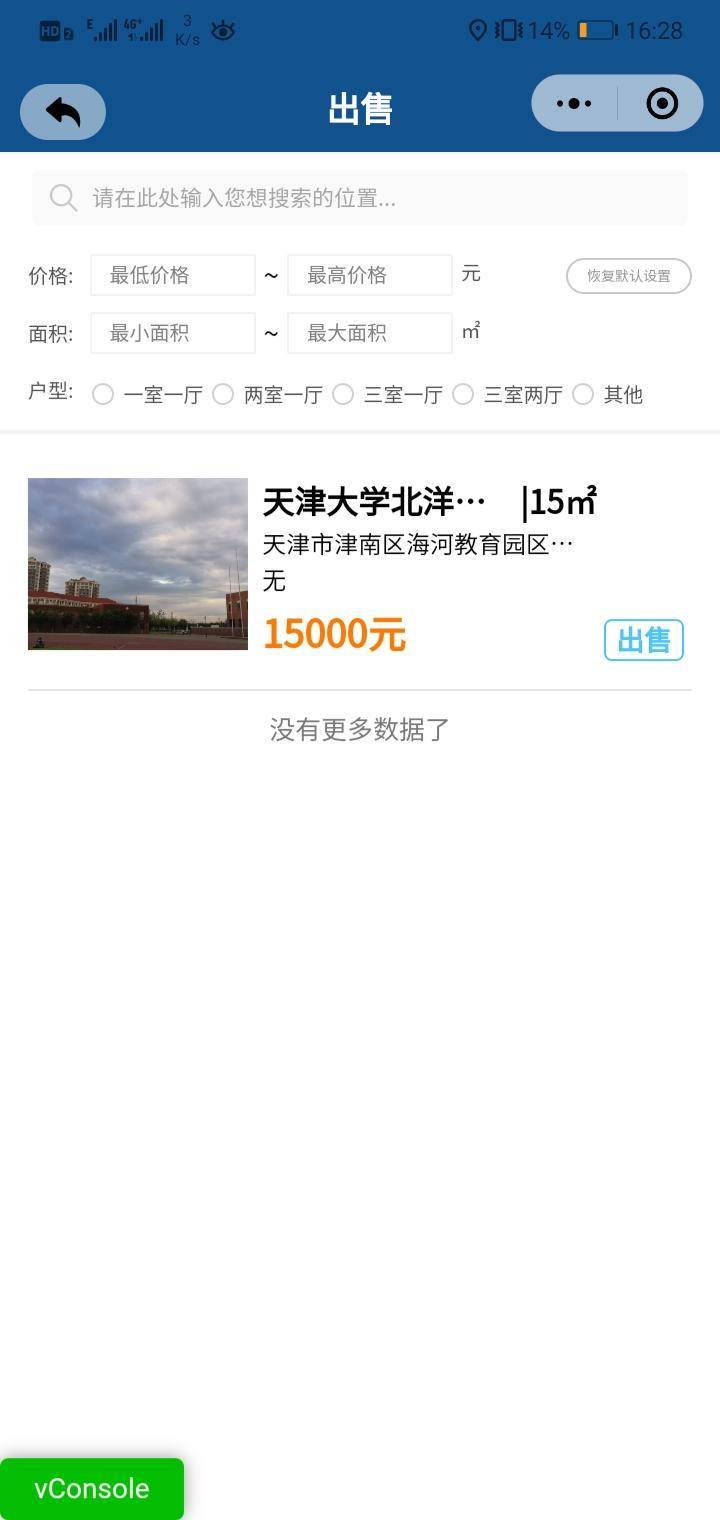
\includegraphics[width=3.8cm,height=8cm]{test/image/test11.png} 
       \caption{出售界面} 
        \end{minipage}
    \begin{minipage}[t]{0.32\textwidth}
    \centering
    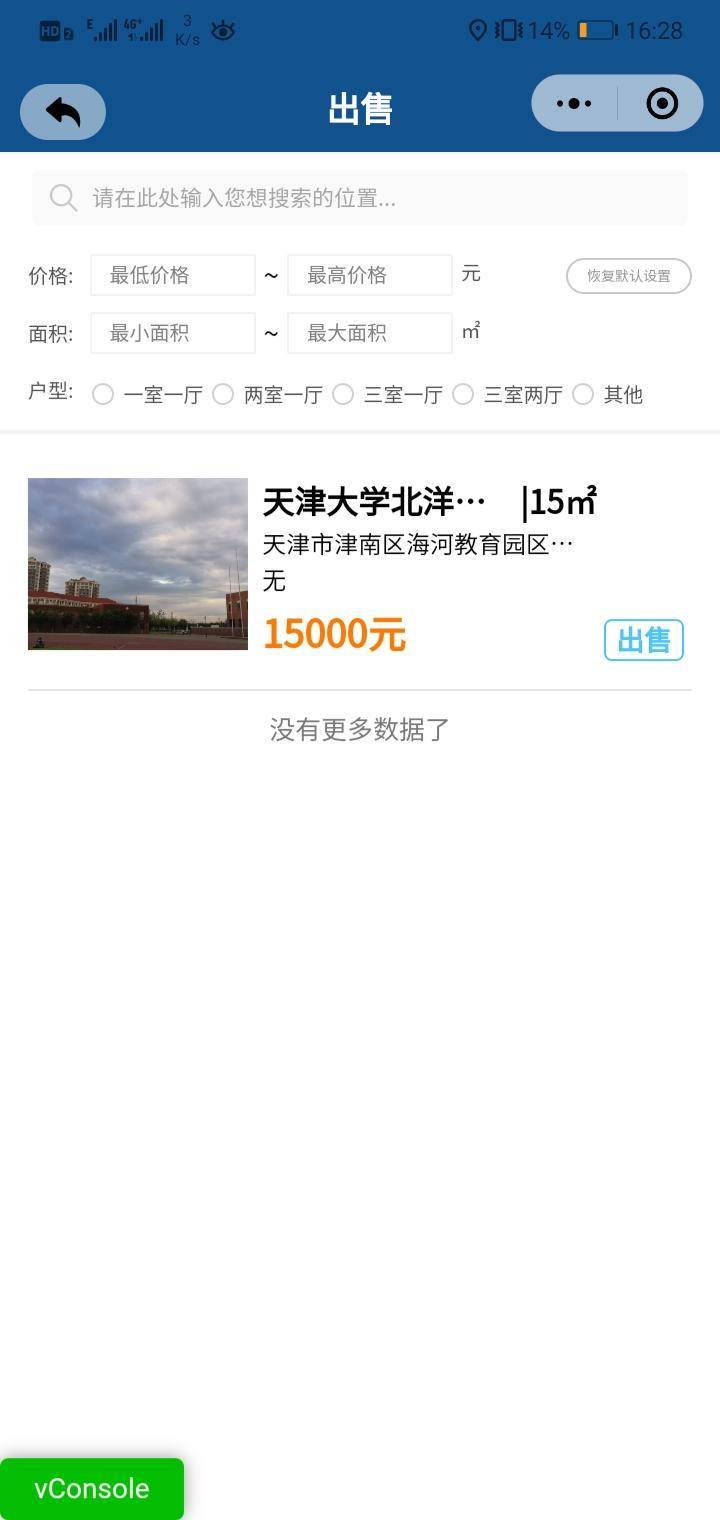
\includegraphics[width=3.8cm,height=8cm]{test/image/test11.png} 
   \caption{出售界面} 
    \end{minipage}
    \begin{minipage}[t]{0.32\textwidth}
    \centering
    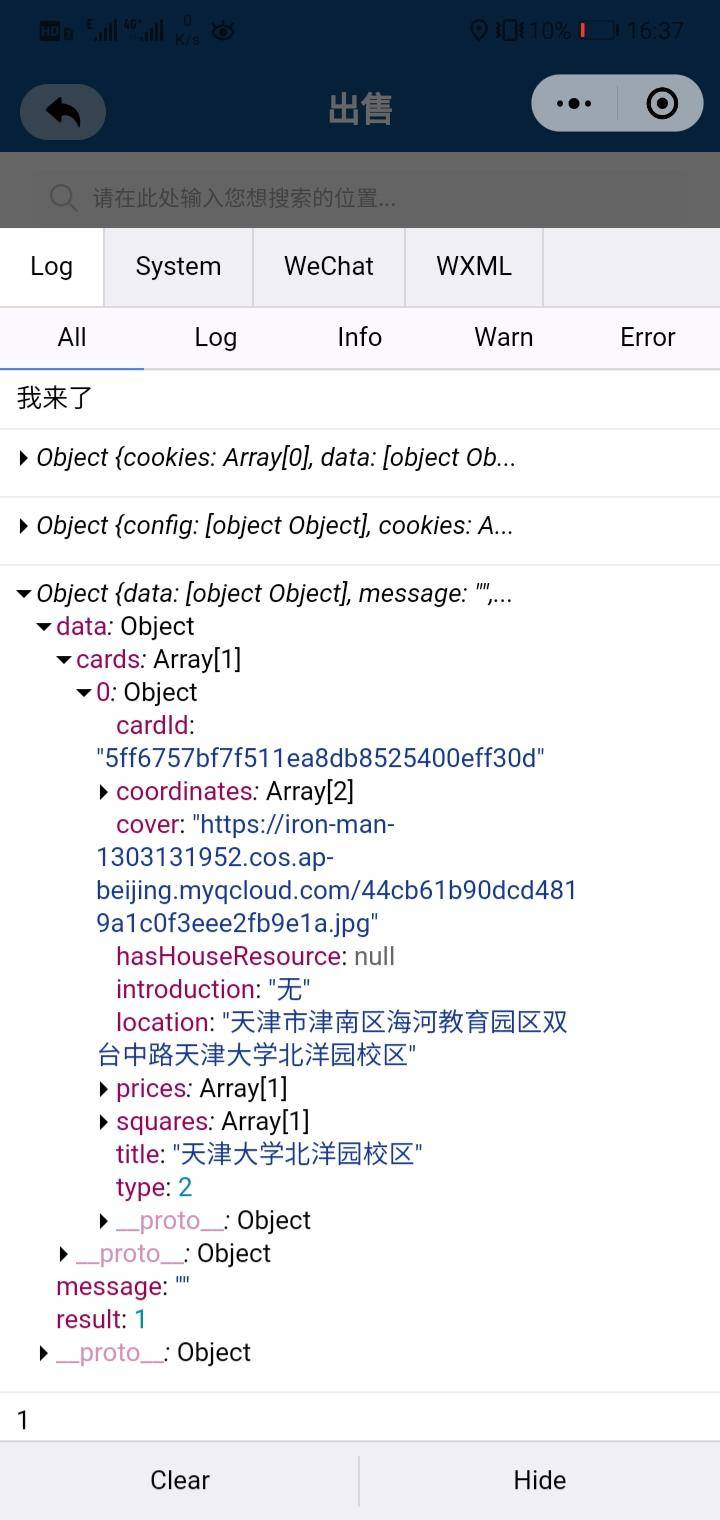
\includegraphics[width=3.8cm,height=8cm]{test/image/test12.png}
    \caption{测试结果}
    \end{minipage}
    \end{figure}
 
\section{查看求租帖子功能测试}
实现用例1:房屋信息查询

功能描述:用户可指定查看求租类型的帖子

用户操作:在“首页”页面下,点击求租

预期结果:服务器返回求租帖子数据,进入求租帖子查询界面

测试结果:通过
\begin{figure}[htbp]
    \centering
    \begin{minipage}[t]{0.32\textwidth}
        \centering
        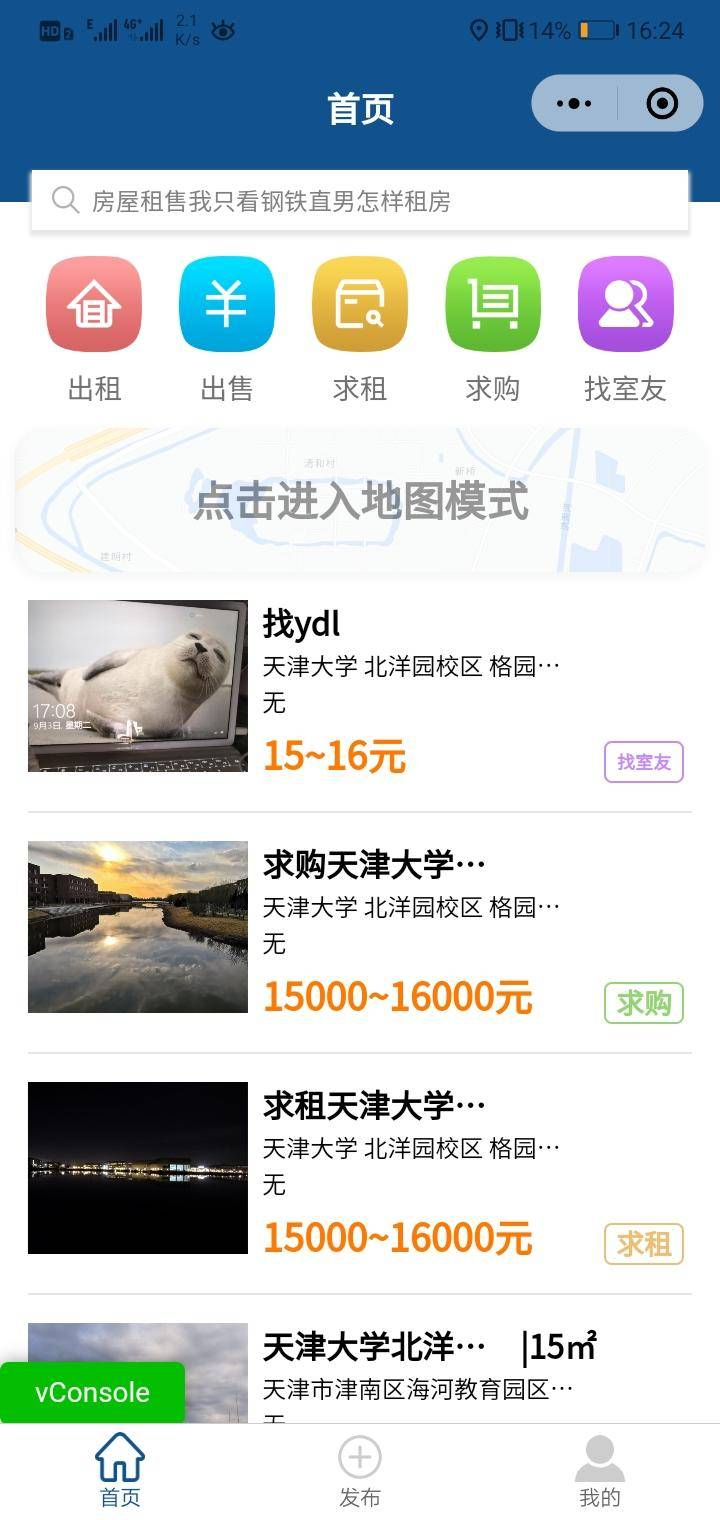
\includegraphics[width=3.8cm,height=8cm]{test/image/test13.png} 
       \caption{求租界面} 
        \end{minipage}
    \begin{minipage}[t]{0.32\textwidth}
    \centering
    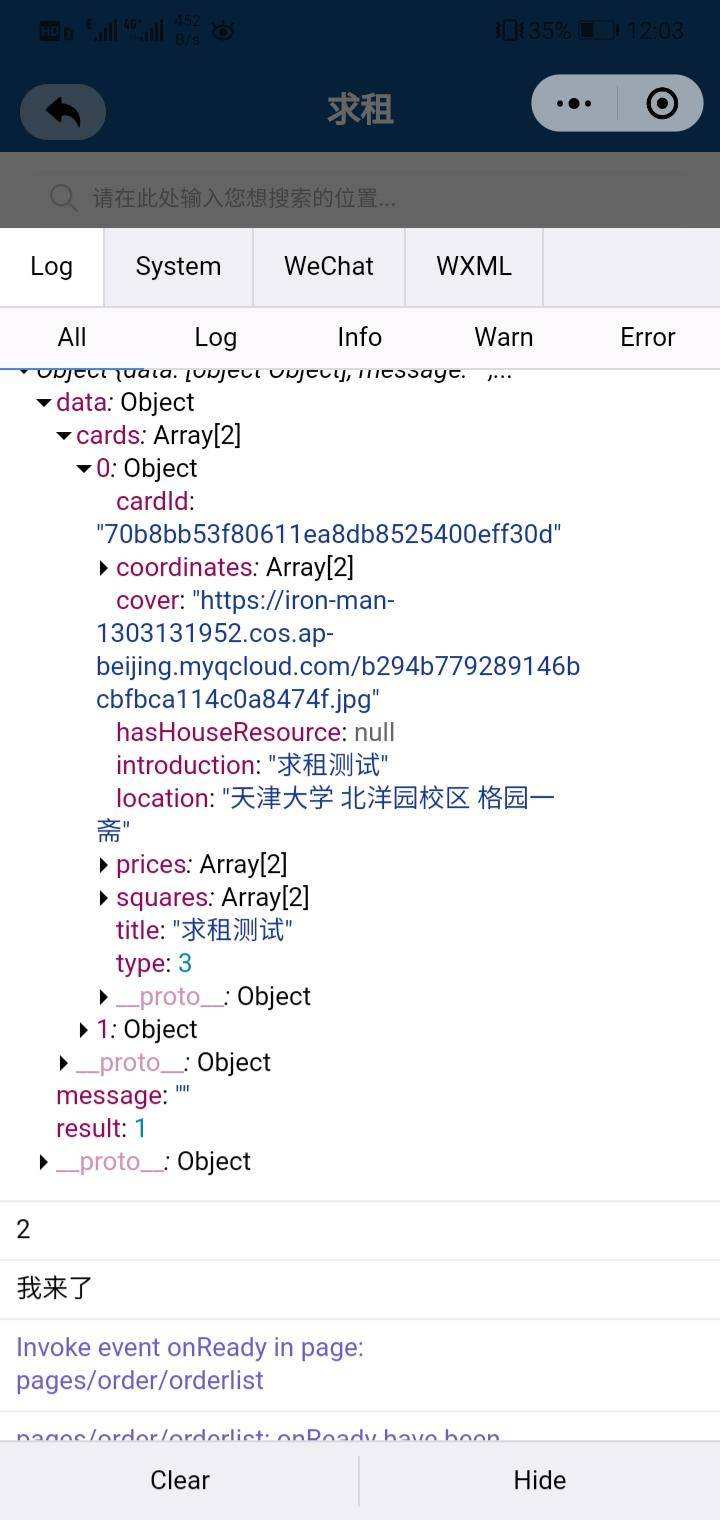
\includegraphics[width=3.8cm,height=8cm]{test/image/test14.png} 
   \caption{求租界面} 
    \end{minipage}
    \begin{minipage}[t]{0.32\textwidth}
    \centering
    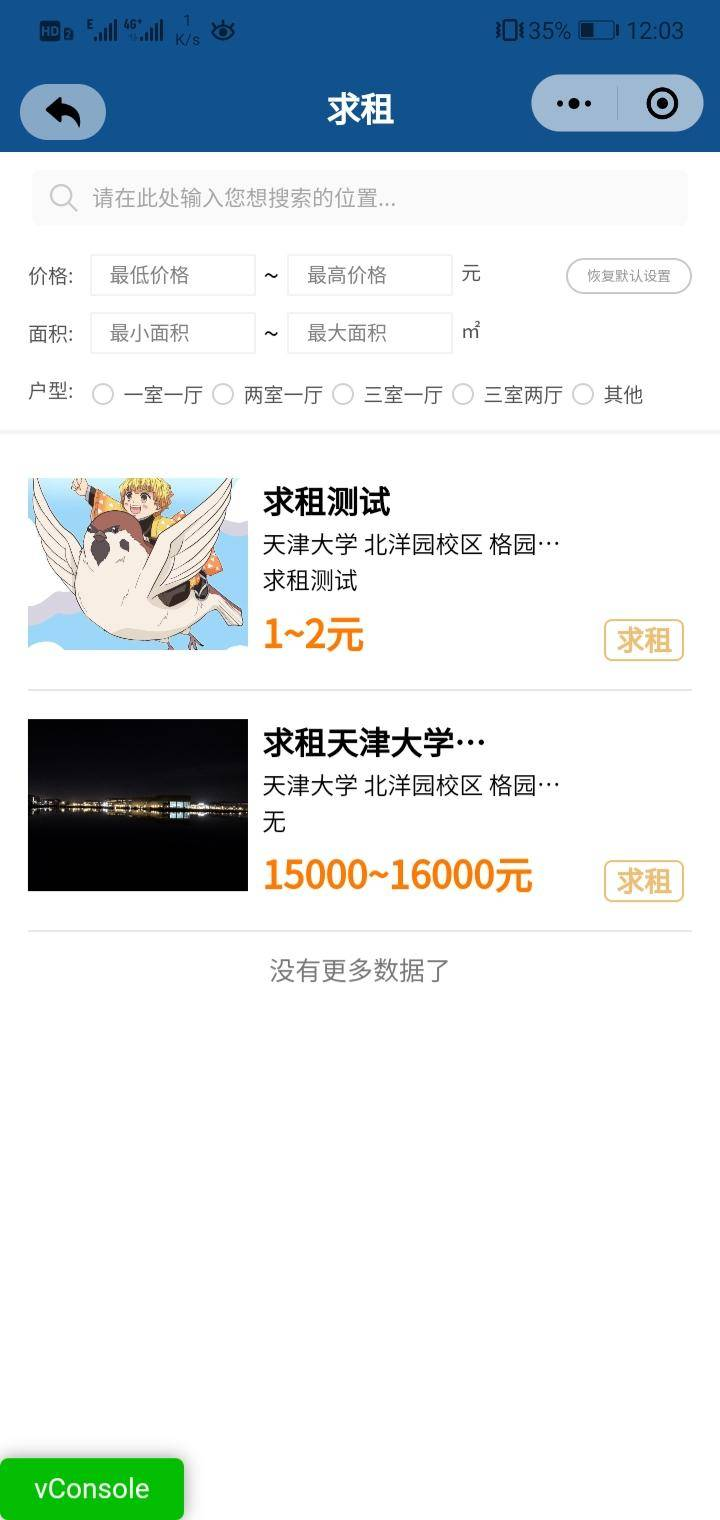
\includegraphics[width=3.8cm,height=8cm]{test/image/test15.png}
    \caption{测试结果}
    \end{minipage}
    \end{figure}
  
\section{查看求购帖子功能测试}
实现用例1:房屋信息查询

功能描述:用户可指定查看求售类型的帖子

用户操作:在“首页”页面下,点击求售

预期结果:服务器返回求售帖子数据,进入求售帖子查询界面

测试结果:通过
\newpage
\begin{figure}[htbp]
    \centering
    \begin{minipage}[t]{0.32\textwidth}
        \centering
        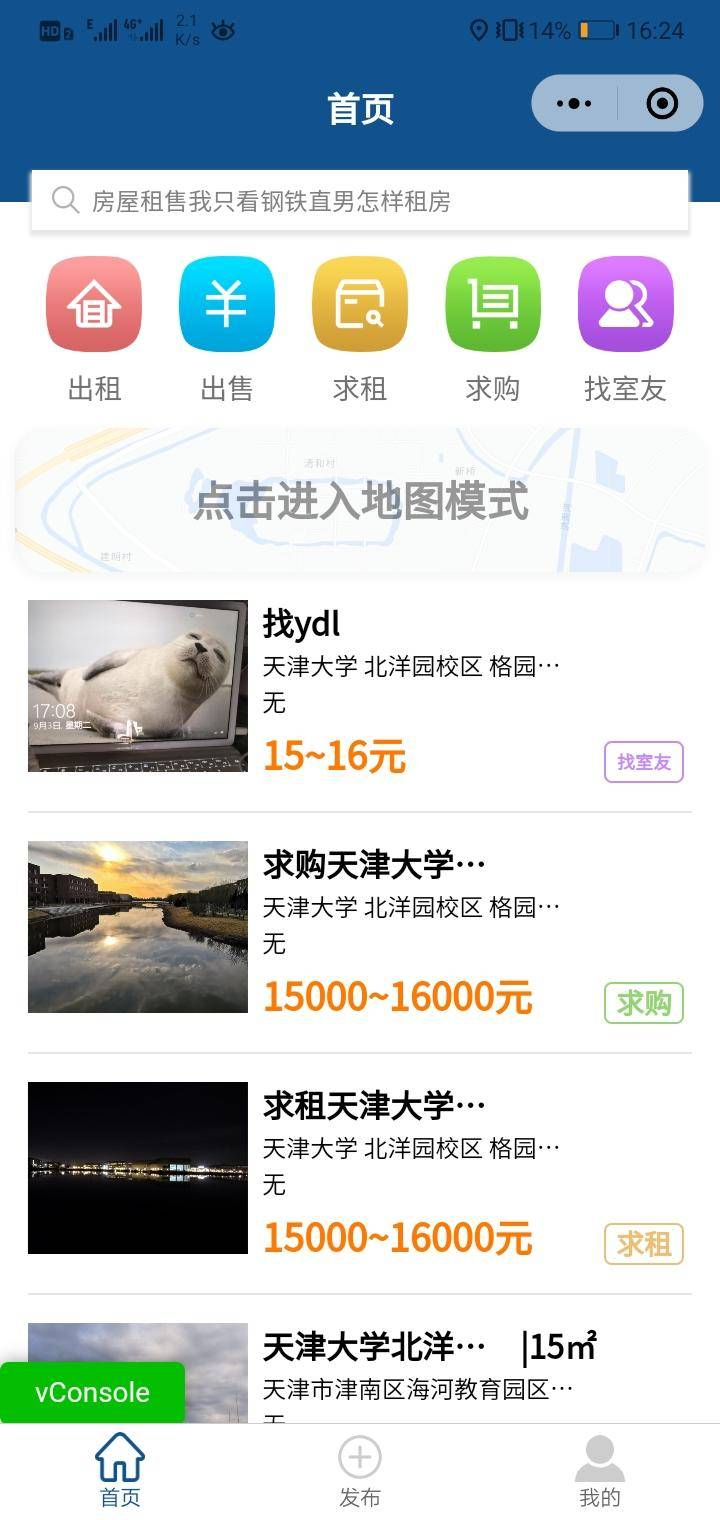
\includegraphics[width=3.8cm,height=8cm]{test/image/test13.png} 
       \caption{求购界面} 
        \end{minipage}
    \begin{minipage}[t]{0.32\textwidth}
    \centering
    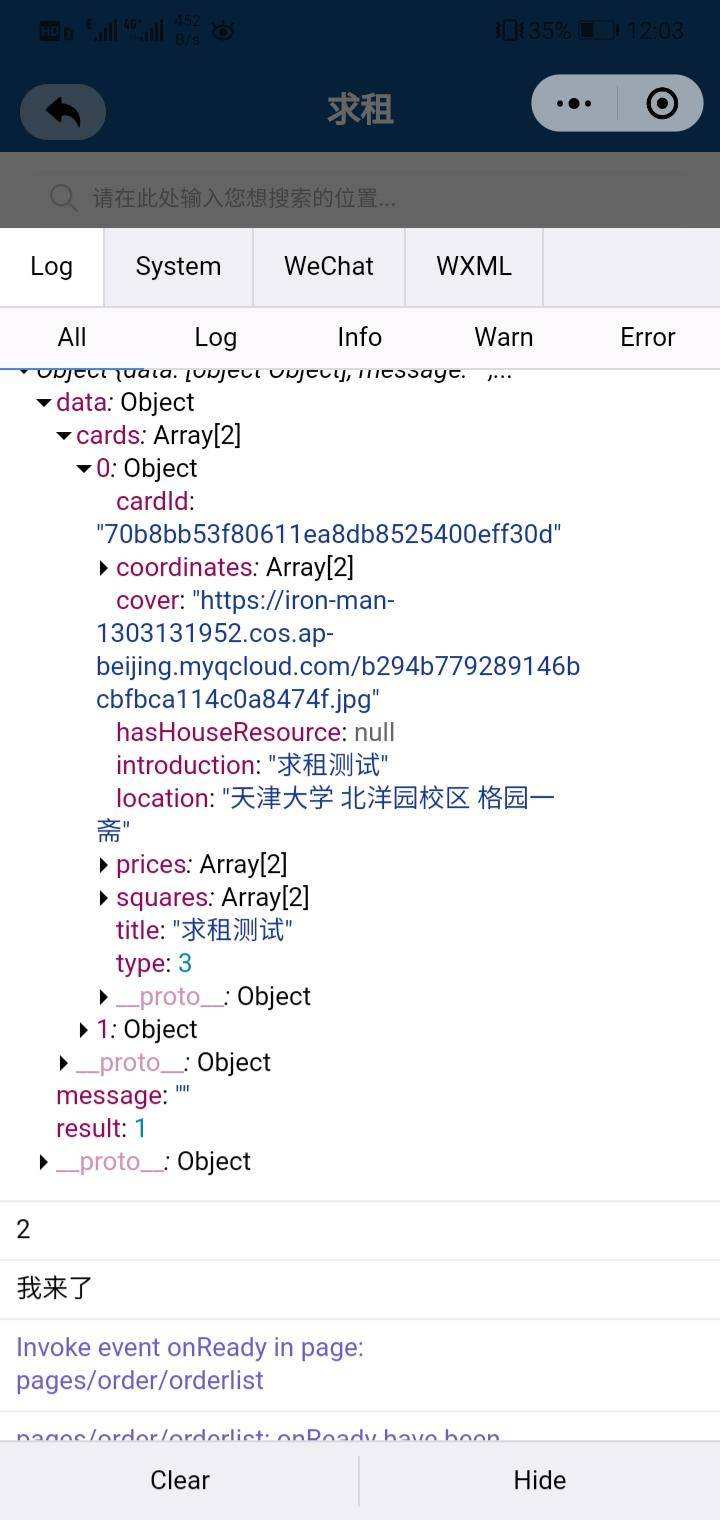
\includegraphics[width=3.8cm,height=8cm]{test/image/test14.png} 
   \caption{求购界面} 
    \end{minipage}
    \begin{minipage}[t]{0.32\textwidth}
    \centering
    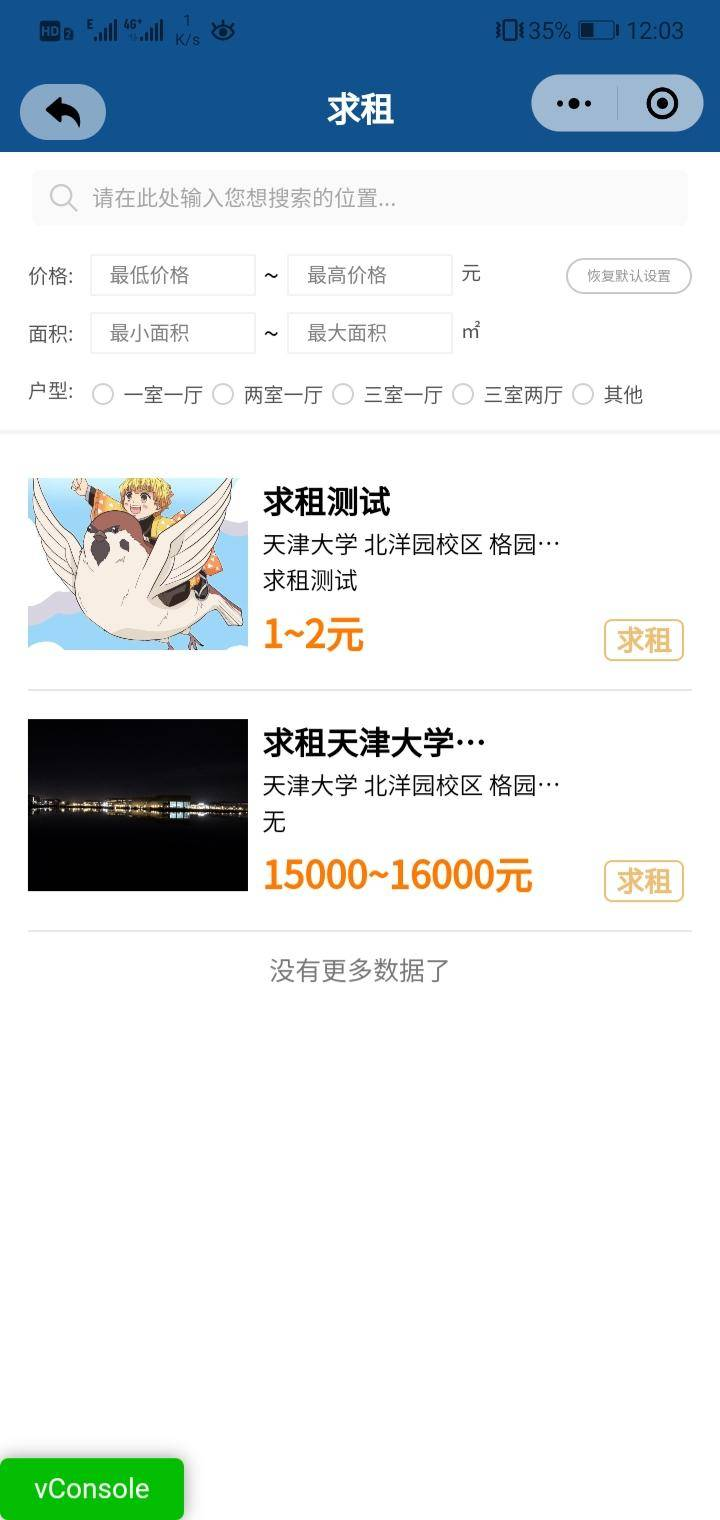
\includegraphics[width=3.8cm,height=8cm]{test/image/test15.png}
    \caption{测试结果}
    \end{minipage}
    \end{figure}

\section{查看求租找室友帖子功能测试}
实现用例1:房屋信息查询

功能描述:用户可指定查看找室友类型的帖子

用户操作:在“首页”页面下,点击找室友

预期结果:服务器返回找室友帖子数据,进入找室友帖子查询界面

测试结果:通过
\begin{figure}[htbp]
    \centering
    \begin{minipage}[t]{0.32\textwidth}
        \centering
        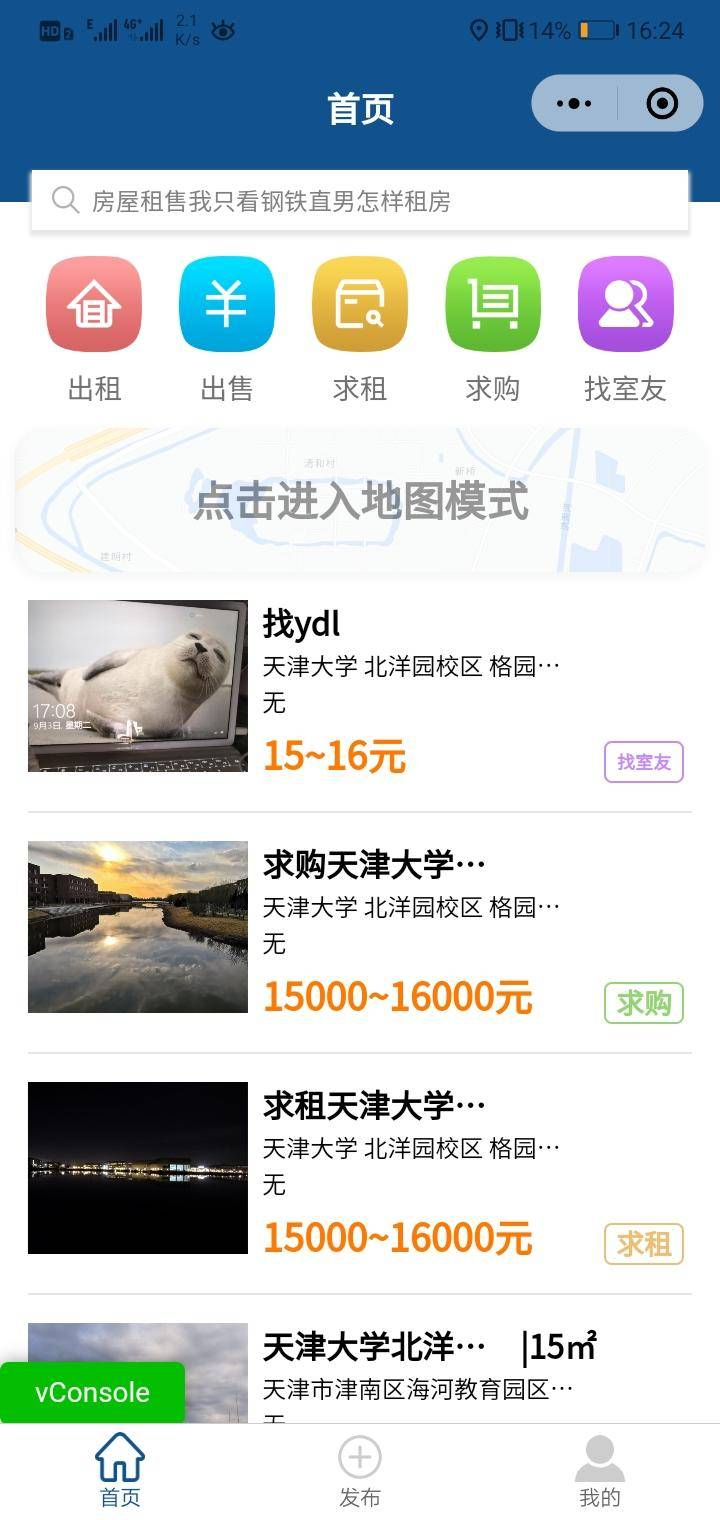
\includegraphics[width=3.8cm,height=8cm]{test/image/test16.png} 
       \caption{找室友界面} 
        \end{minipage}
    \begin{minipage}[t]{0.32\textwidth}
    \centering
    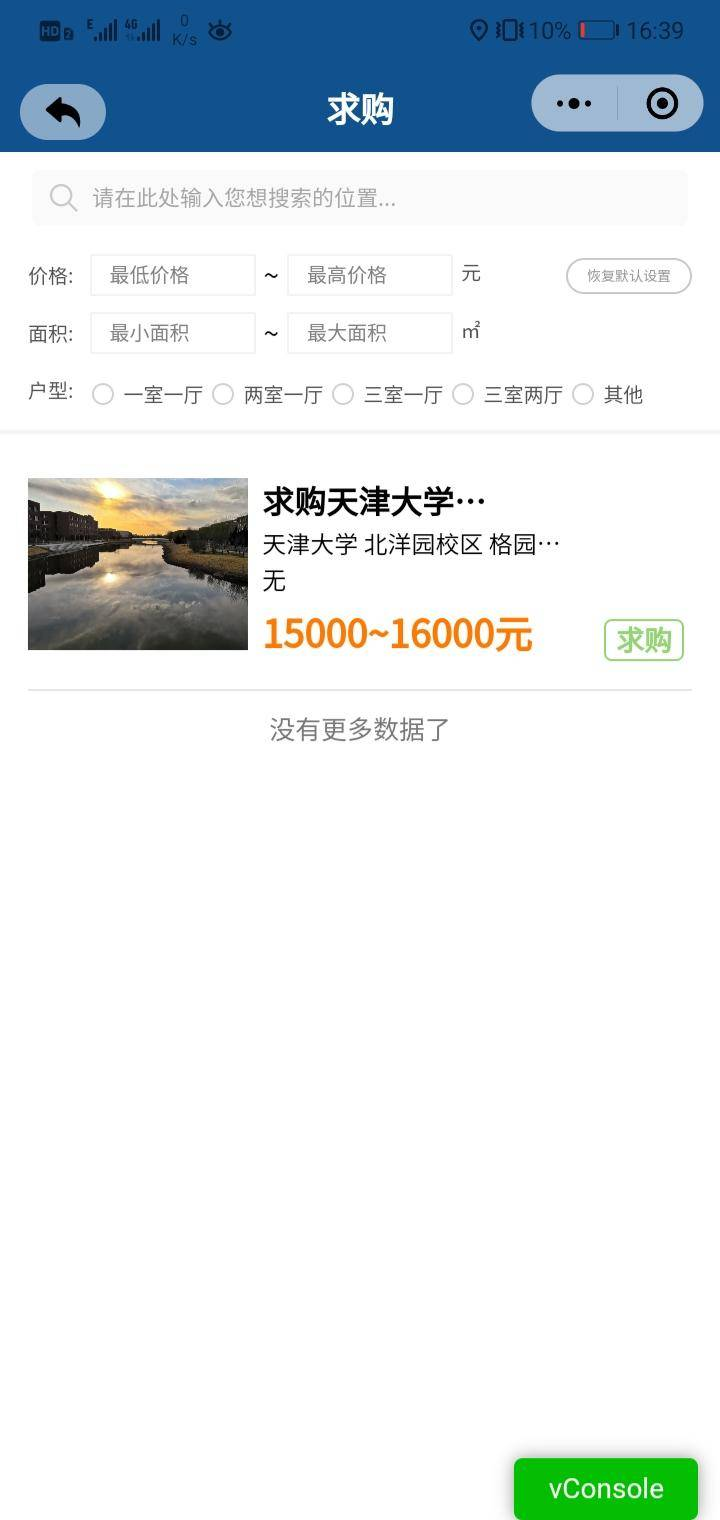
\includegraphics[width=3.8cm,height=8cm]{test/image/test17.png} 
   \caption{找室友界面} 
    \end{minipage}
    \begin{minipage}[t]{0.32\textwidth}
    \centering
    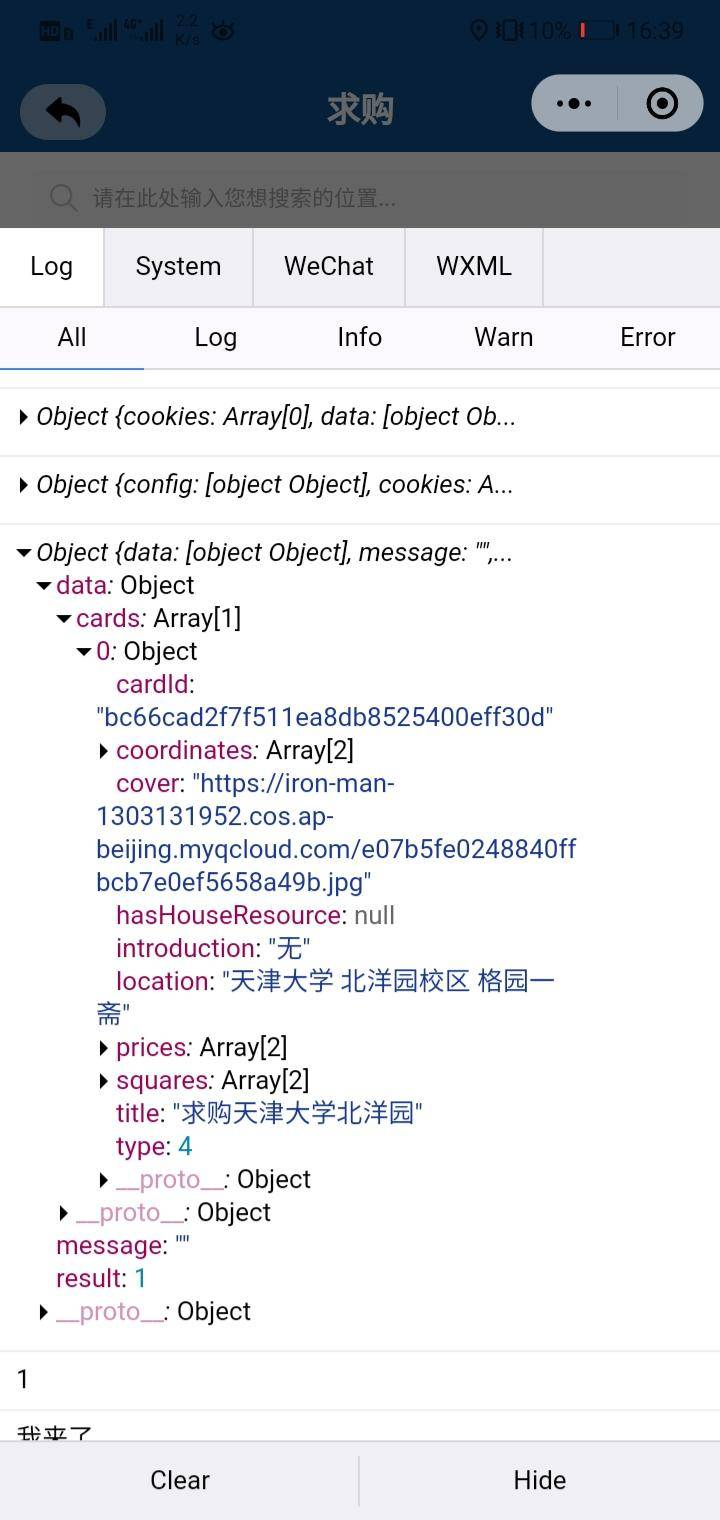
\includegraphics[width=3.8cm,height=8cm]{test/image/test18.png}
    \caption{测试结果}
    \end{minipage}
    \end{figure}
   \newpage 

\section{搜索帖子功能测试}

实现用例1:房屋信息查询

功能描述:用户可以通过地区字段搜索相关的帖子

用户操作:在“搜索“界面 选择帖子类型 输入地区字段 点击搜索

预期结果:服务器返回找室友帖子数据,进入找室友帖子查询界面

测试结果:通过
\begin{figure}[htbp]
    \centering
    \begin{minipage}[t]{0.32\textwidth}
        \centering
        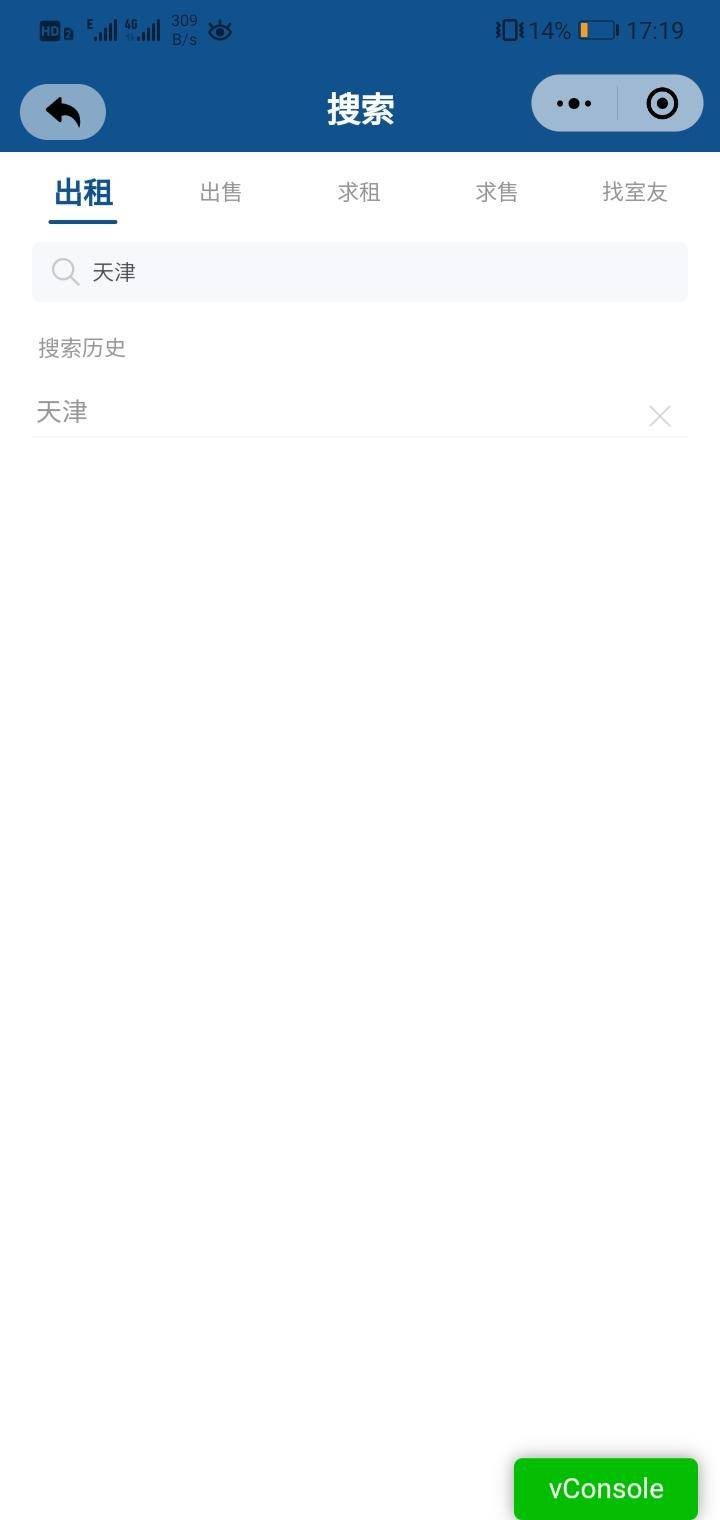
\includegraphics[width=3.8cm,height=8cm]{test/image/test19.png} 
       \caption{搜索界面} 
        \end{minipage}
    \begin{minipage}[t]{0.32\textwidth}
    \centering
    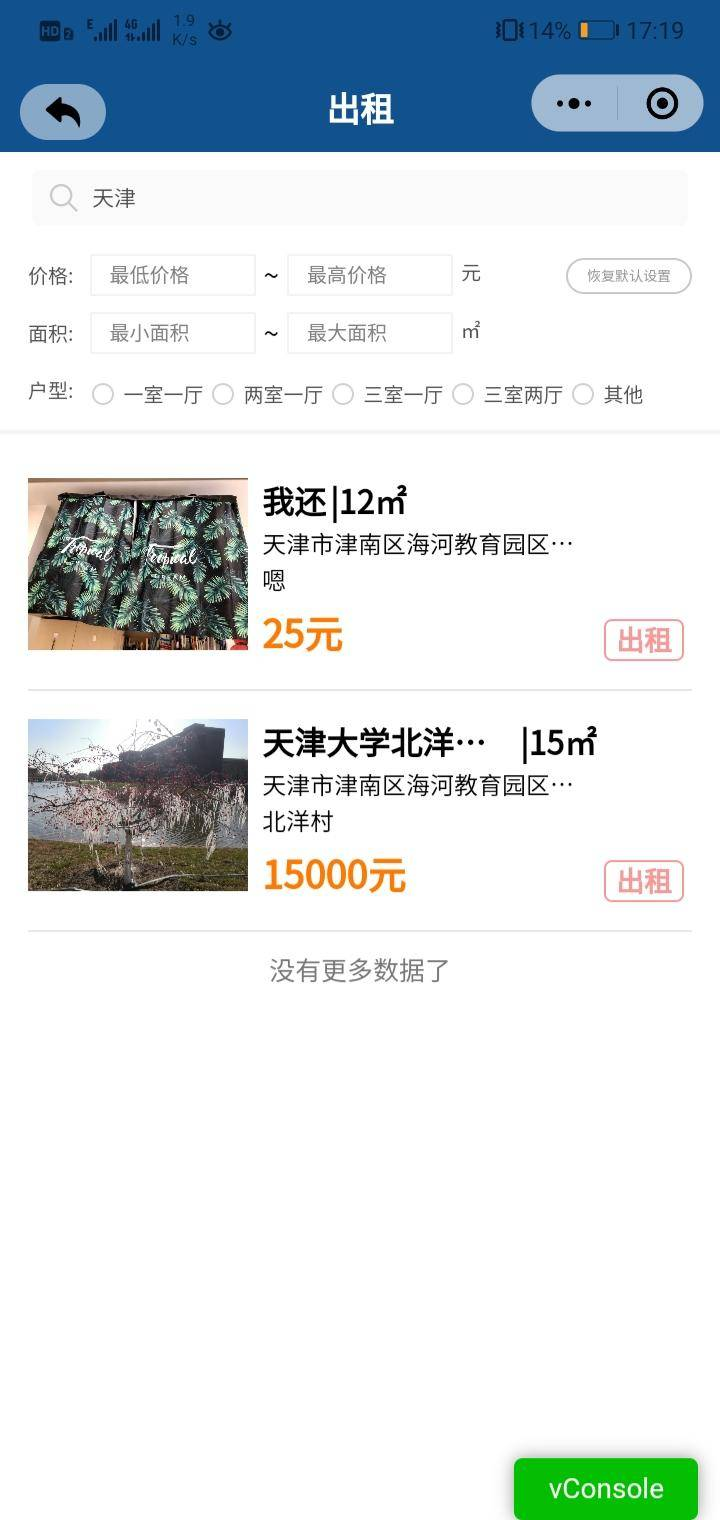
\includegraphics[width=3.8cm,height=8cm]{test/image/test20.png} 
   \caption{搜索结果界面} 
    \end{minipage}
    \begin{minipage}[t]{0.32\textwidth}
    \centering
    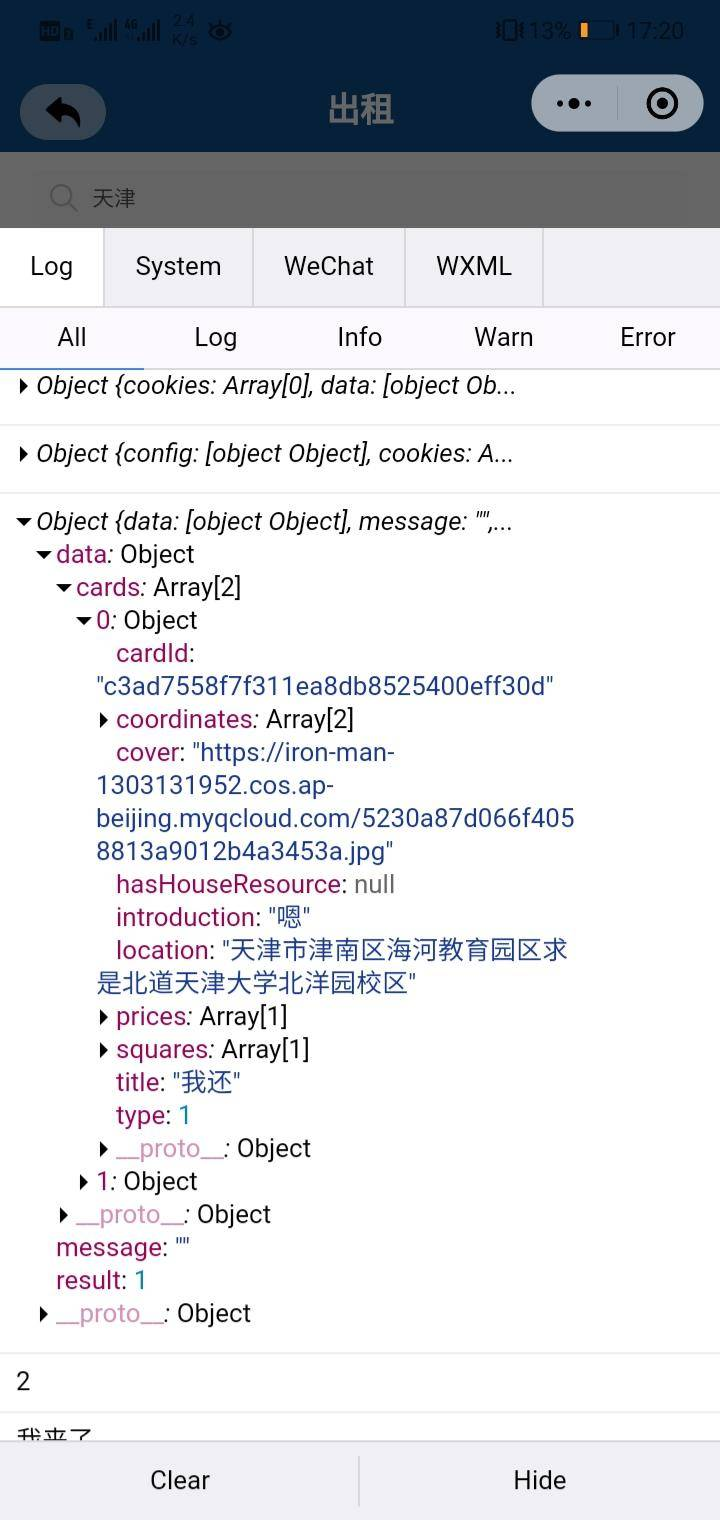
\includegraphics[width=3.8cm,height=8cm]{test/image/test21.png}
    \caption{测试结果}
    \end{minipage}
    \end{figure}

\section{按价格面积户型搜索帖子功能测试}
实现用例1:房屋信息查询

功能描述:用户可以通过价格面积字段搜索相关的帖子

用户操作:在“出租“界面 输入价格区间 面积区间 户型

预期结果:服务器返回指定类型的帖子数据列表展示出符合条件的帖子

测试结果:通过
\newpage
\begin{figure}[htbp]
    \centering
    \begin{minipage}[t]{0.32\textwidth}
        \centering
        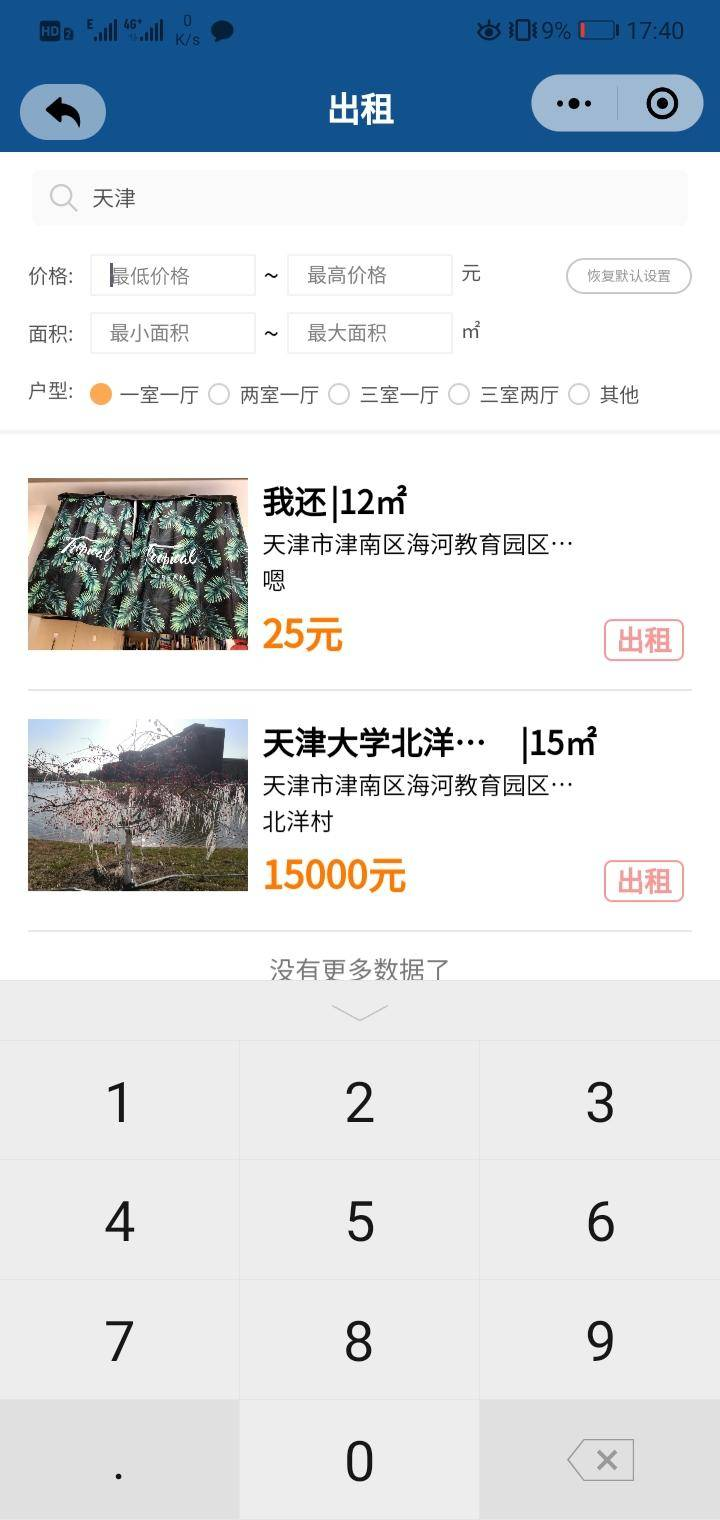
\includegraphics[width=3.8cm,height=8cm]{test/image/test22.png} 
       \caption{输入搜索条件} 
        \end{minipage}
    \begin{minipage}[t]{0.32\textwidth}
    \centering
    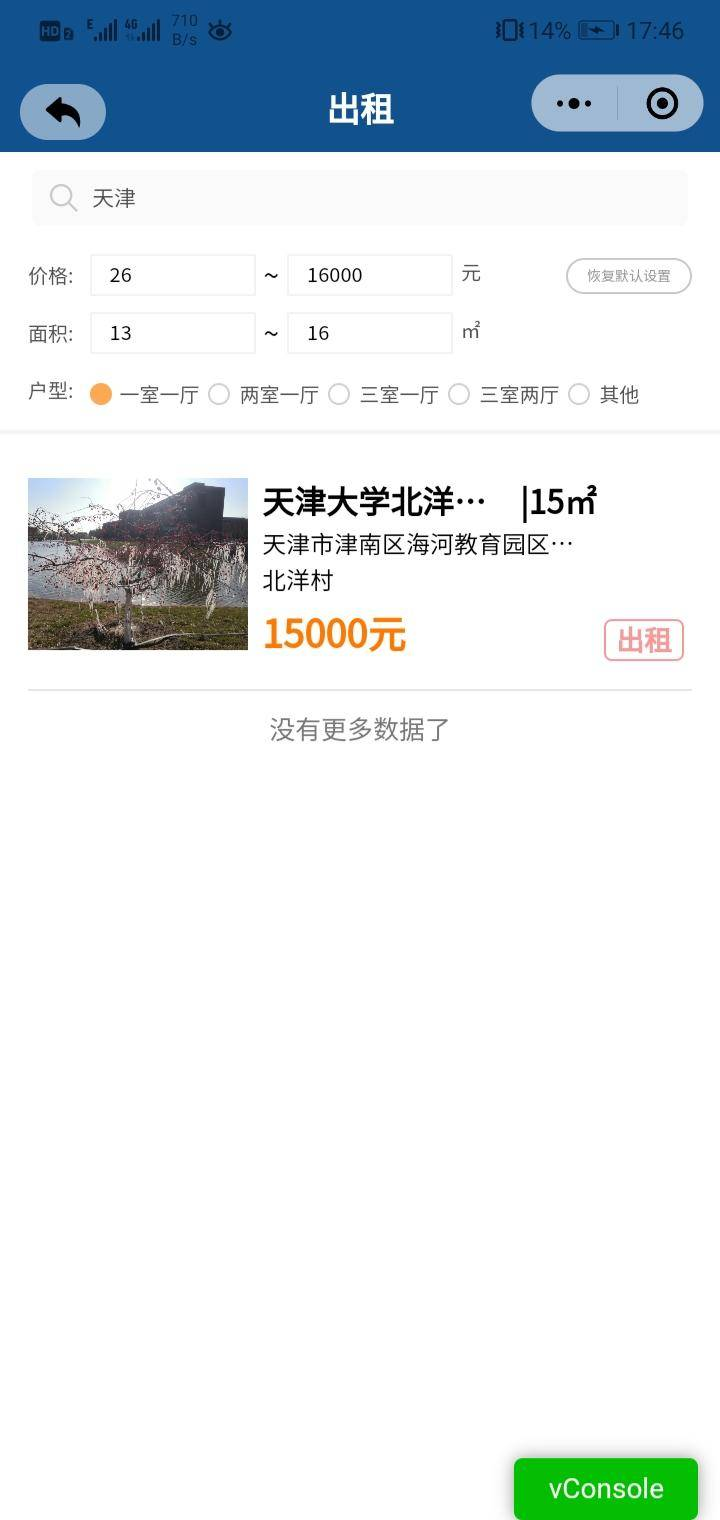
\includegraphics[width=3.8cm,height=8cm]{test/image/test23.png} 
   \caption{搜索结果} 
    \end{minipage}
    \begin{minipage}[t]{0.32\textwidth}
    \centering
    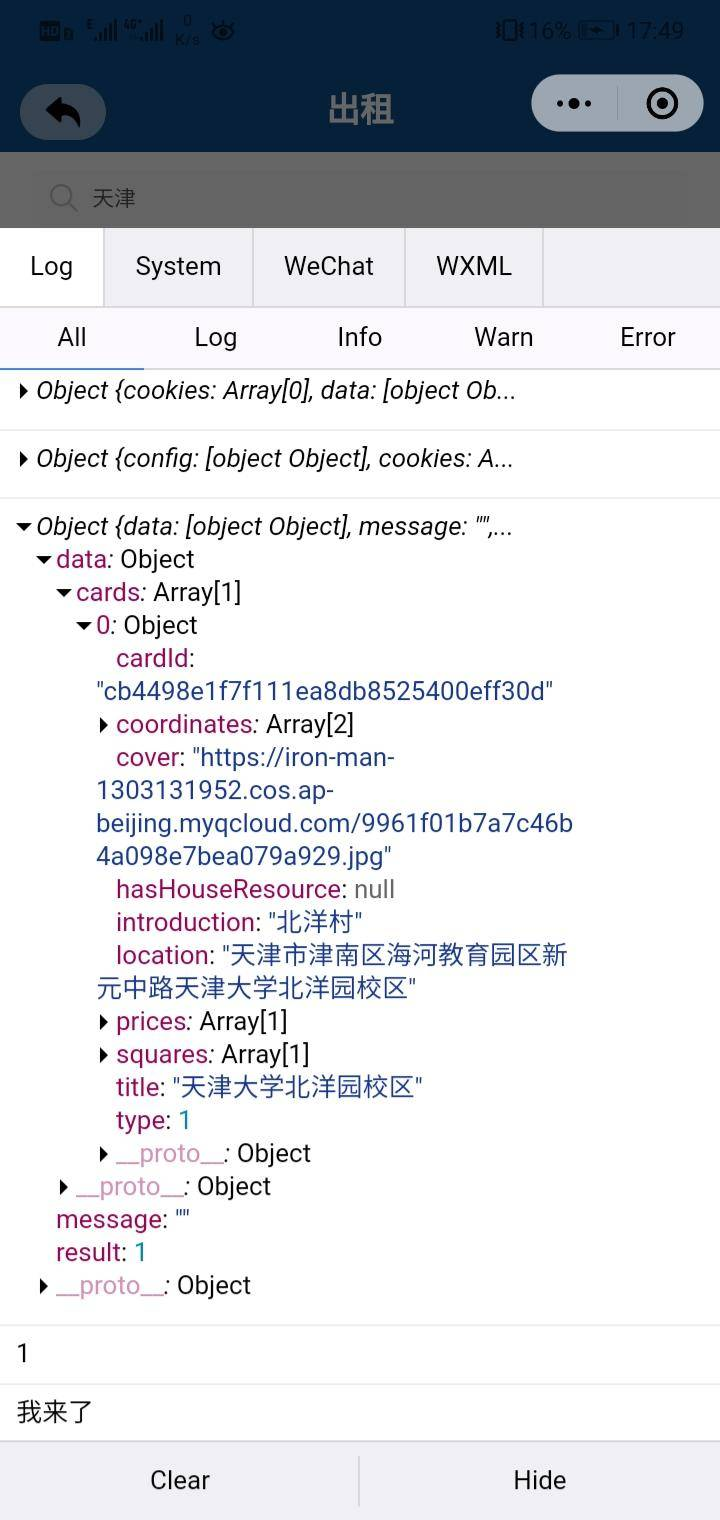
\includegraphics[width=3.8cm,height=8cm]{test/image/test24.png}
    \caption{测试结果}
    \end{minipage}
    \end{figure}
   
\section{帖子详情功能测试}
实现用例1:房屋信息查询

功能描述:用户可以查看帖子的详细信息

用户操作:点击帖子列表中的帖子,可进入对应帖子的详情页

预期结果:页面跳转到”首页“

测试结果:通过
\begin{figure}[htbp]
    \centering
    \begin{minipage}[t]{0.48\textwidth}
        \centering
        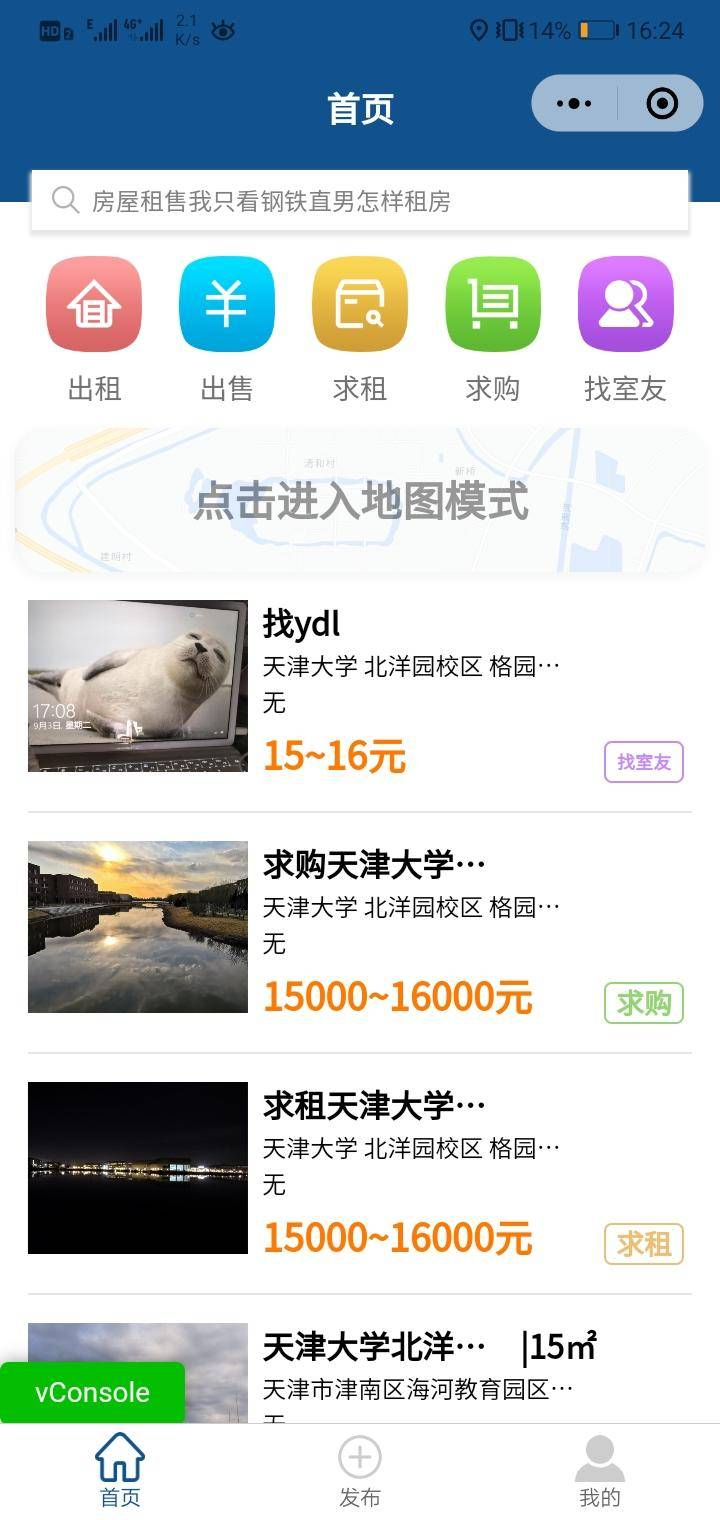
\includegraphics[width=4cm,height=8cm]{test/image/test16.png} 
       \caption{查看帖子详情} 
        \end{minipage}
   
    \end{figure}
   \newpage 
\section{发布出租帖子功能测试}

实现用例9:发布房屋出租信息

功能描述:用户可以填写房屋信息和要求,发布房屋出租信息

用户操作:在”发布“界面点击”我要出租“按钮,进入信息填写界面,填写后点击发布

预期结果:页面跳转到”首页“

测试结果:通过
    \begin{figure}[htbp]
        \centering
        \begin{minipage}[t]{0.48\textwidth}
        \centering
        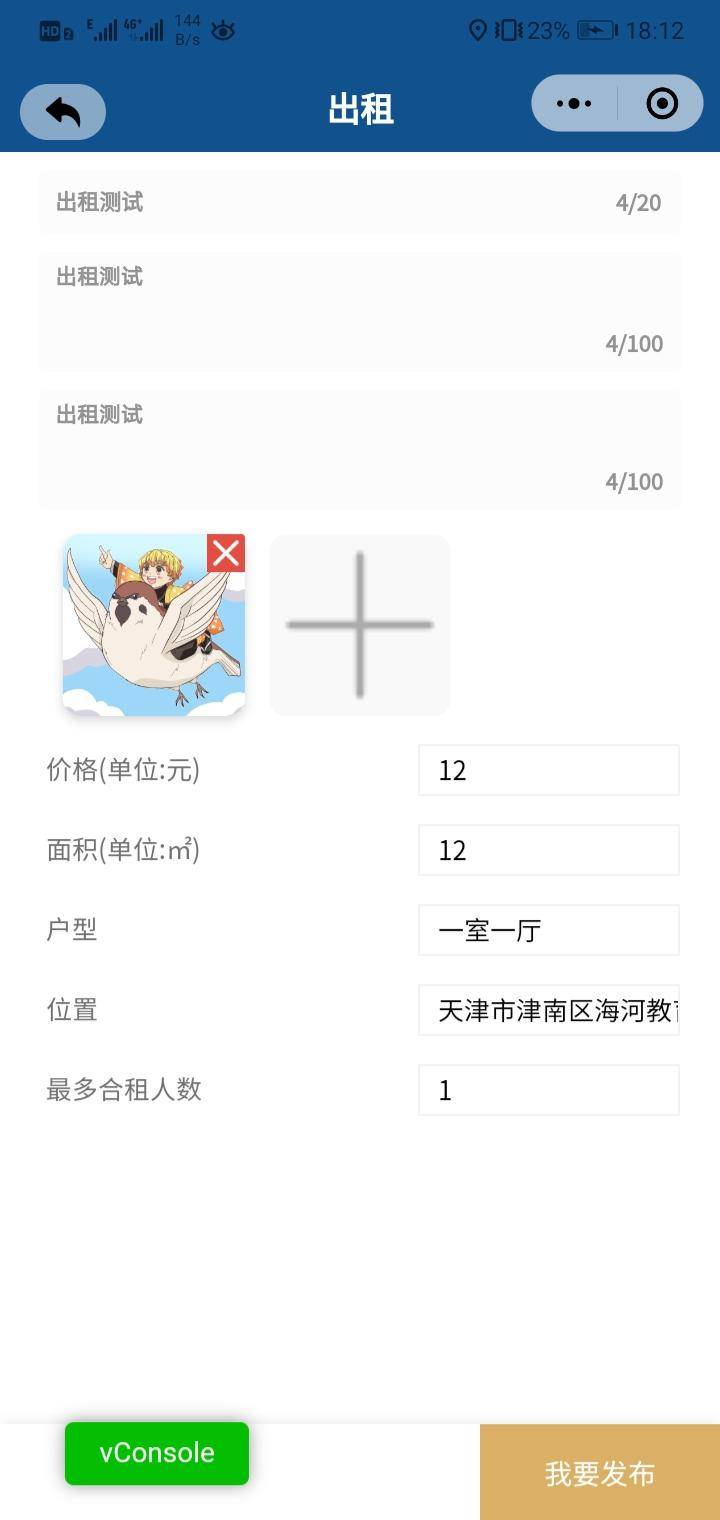
\includegraphics[width=4cm,height=8cm]{test/image/test26.png} 
     
       \caption{发布出租信息} 
        \end{minipage}
        \begin{minipage}[t]{0.48\textwidth}
        \centering
        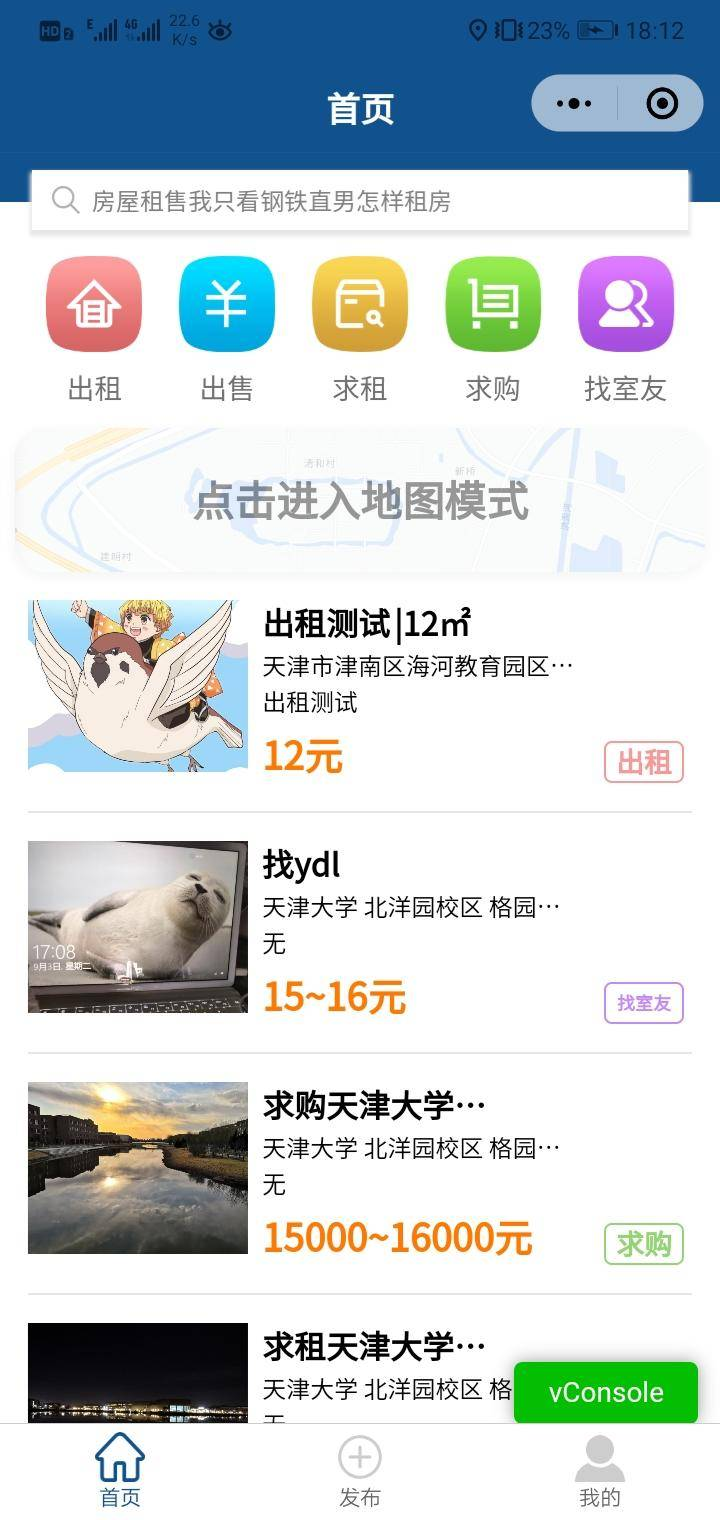
\includegraphics[width=4cm,height=8cm]{test/image/test27.png}
        \caption{测试结果}
        \end{minipage}
        \end{figure}
 
\section{发布出售帖子功能测试}

实现用例5:发布房屋出售信息

功能描述:用户可以填写房屋信息和要求,发布房屋出售信息

用户操作:在”发布“界面点击”我要出售“按钮,进入信息填写界面,填写后点击发布

预期结果:页面跳转到”首页“

测试结果:通过
\newpage 
    \begin{figure}[htbp]
        \centering
        \begin{minipage}[t]{0.48\textwidth}
        \centering
        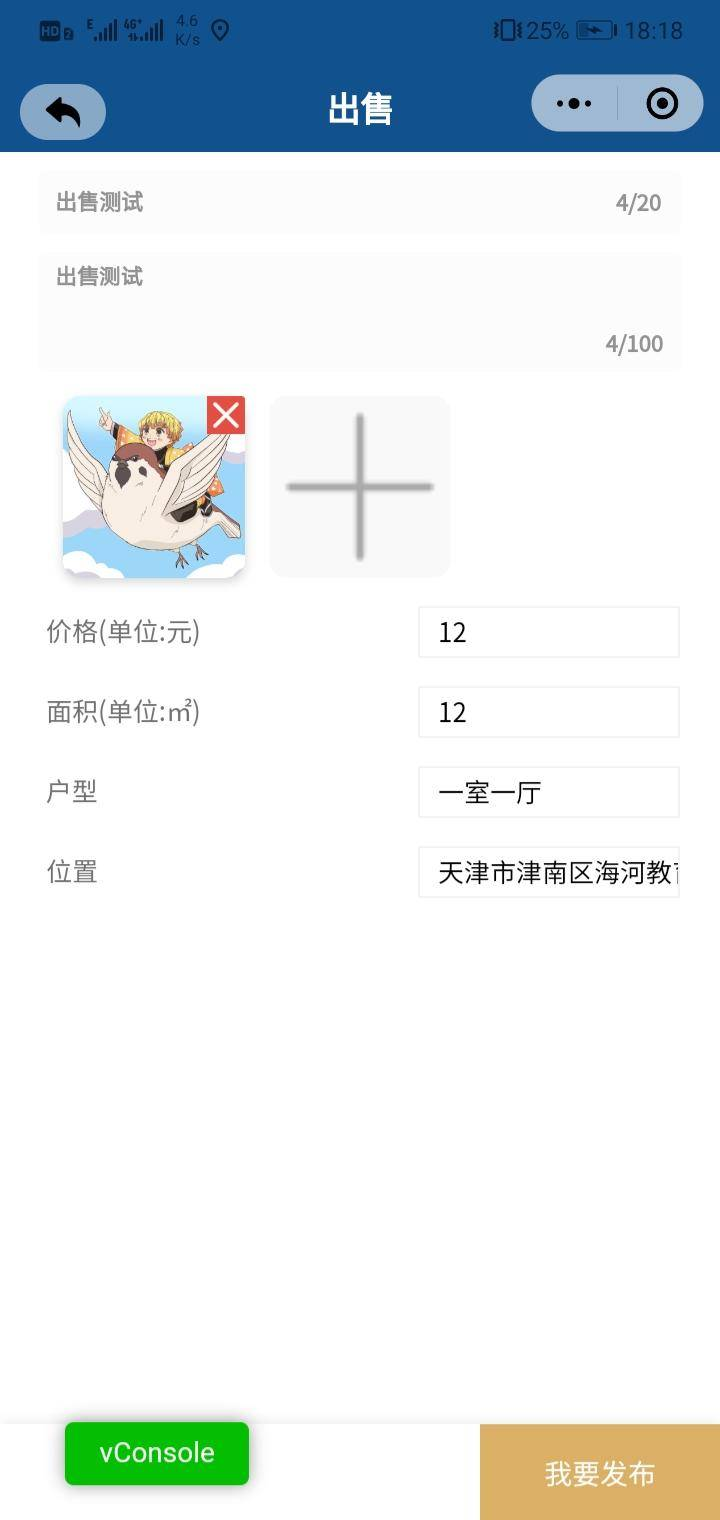
\includegraphics[width=4cm,height=8cm]{test/image/test28.png} 
     
       \caption{发布出售信息} 
        \end{minipage}
        \begin{minipage}[t]{0.48\textwidth}
        \centering
        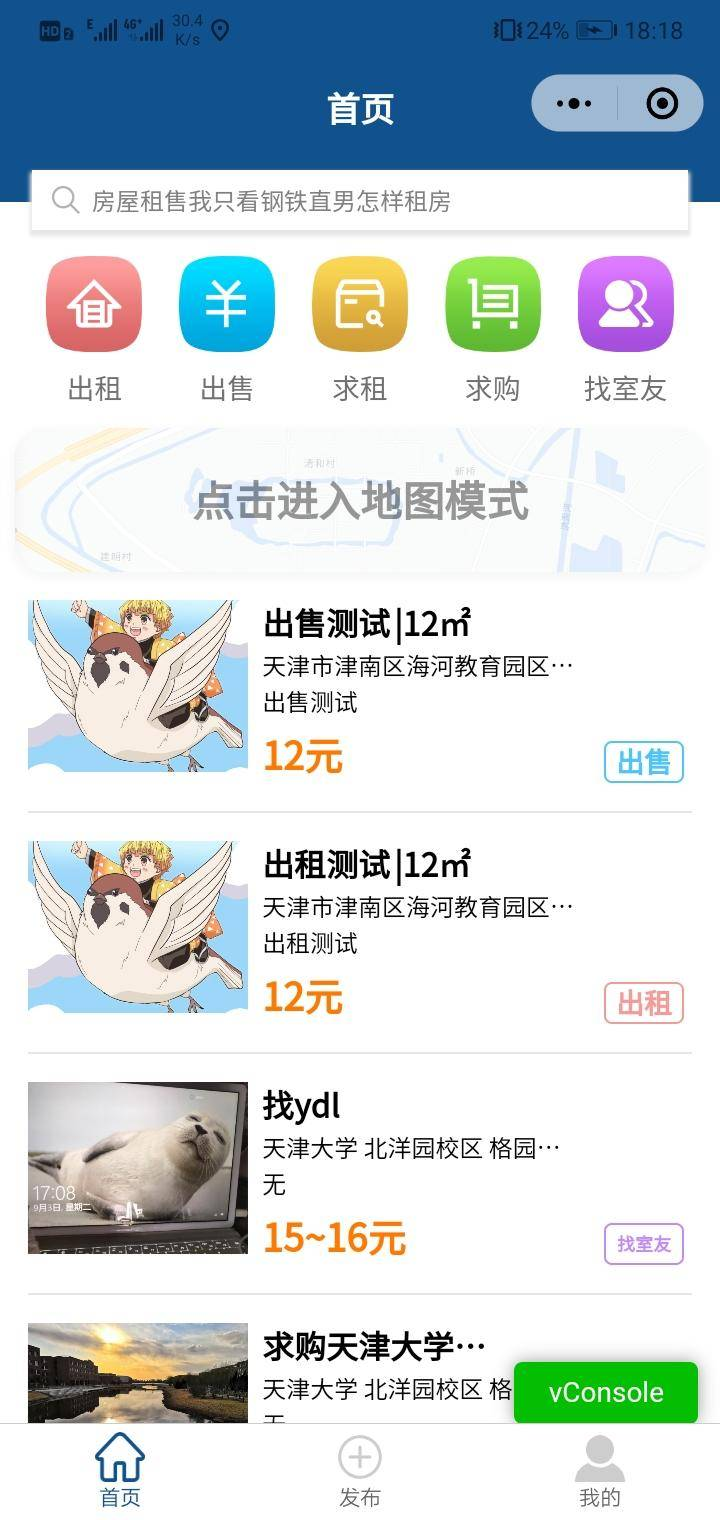
\includegraphics[width=4cm,height=8cm]{test/image/test29.png}
        \caption{测试结果}
        \end{minipage}
        \end{figure}

   \section{发布求租房帖子功能测试}

实现用例12:房屋信息查询

功能描述:用户可以填写对房屋的期望,发布房屋求租信息

用户操作:在”发布“界面点击”我要求租“按钮,进入信息填写界面,填写后点击发布

预期结果:页面跳转到”首页“

测试结果:通过
\begin{figure}[htbp]
    \centering
    \begin{minipage}[t]{0.48\textwidth}
    \centering
    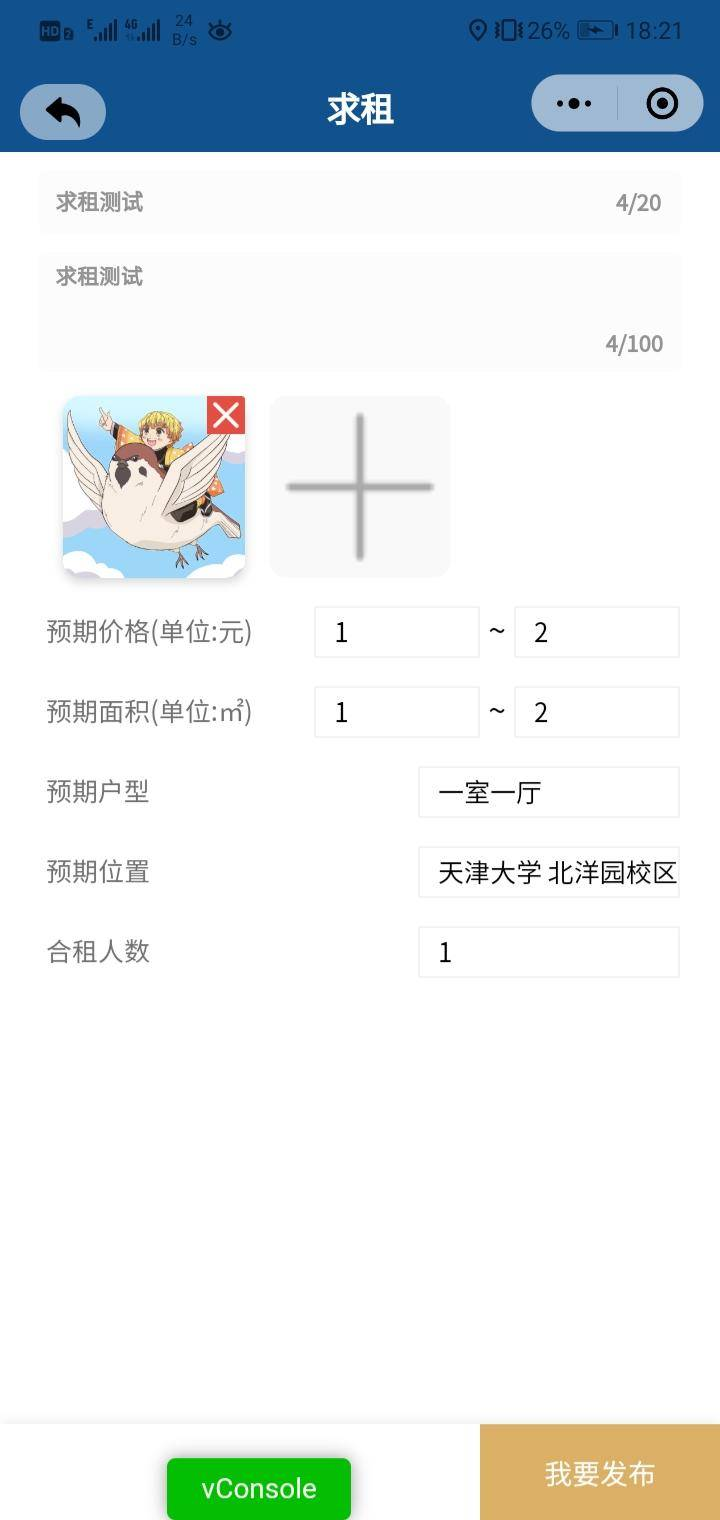
\includegraphics[width=4cm,height=8cm]{test/image/test30.png} 
 
   \caption{发布出售信息} 
    \end{minipage}
    \begin{minipage}[t]{0.48\textwidth}
    \centering
    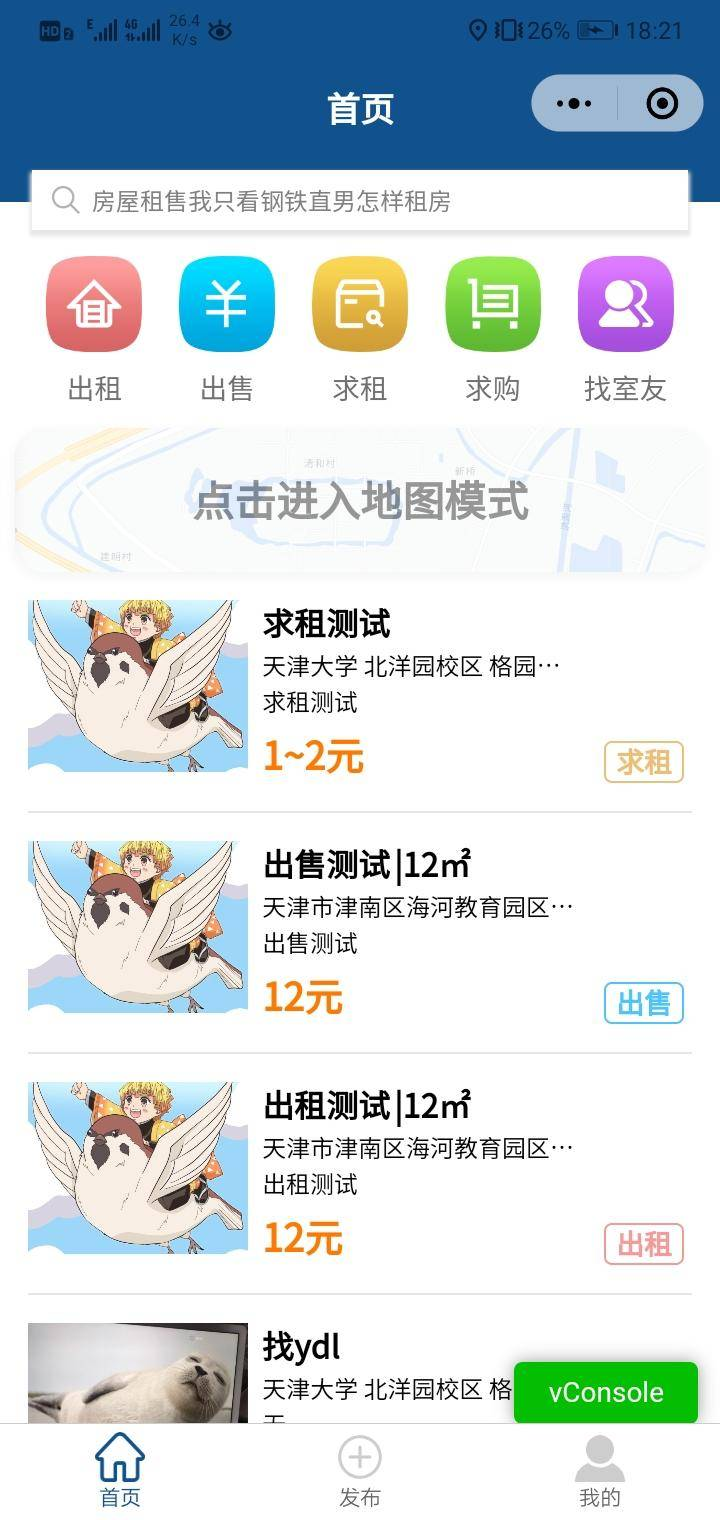
\includegraphics[width=4cm,height=8cm]{test/image/test31.png}
    \caption{测试结果}
    \end{minipage}
    \end{figure}
   \newpage 

   \section{发布求购帖子功能测试}

实现用例14:发出求购信息

功能描述:用户可以填写对房屋的期望,发布房屋求购信息

用户操作:在”发布“界面点击”我要求购“按钮,进入信息填写界面,填写后点击发布

预期结果:页面跳转到”首页“

测试结果:通过
\begin{figure}[htbp]
    \centering
    \begin{minipage}[t]{0.48\textwidth}
    \centering
    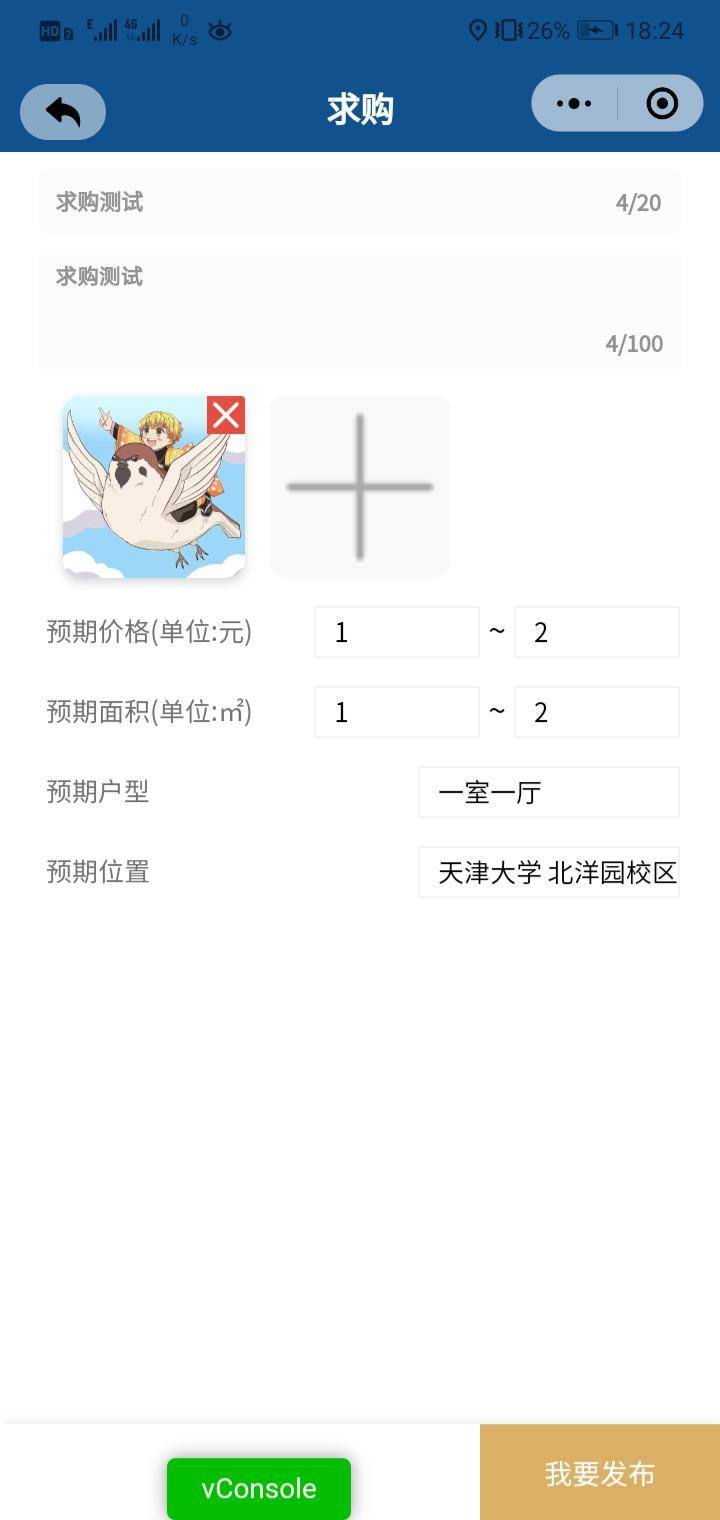
\includegraphics[width=4cm,height=8cm]{test/image/test32.png} 
 
   \caption{发布求购信息} 
    \end{minipage}
    \begin{minipage}[t]{0.48\textwidth}
    \centering
    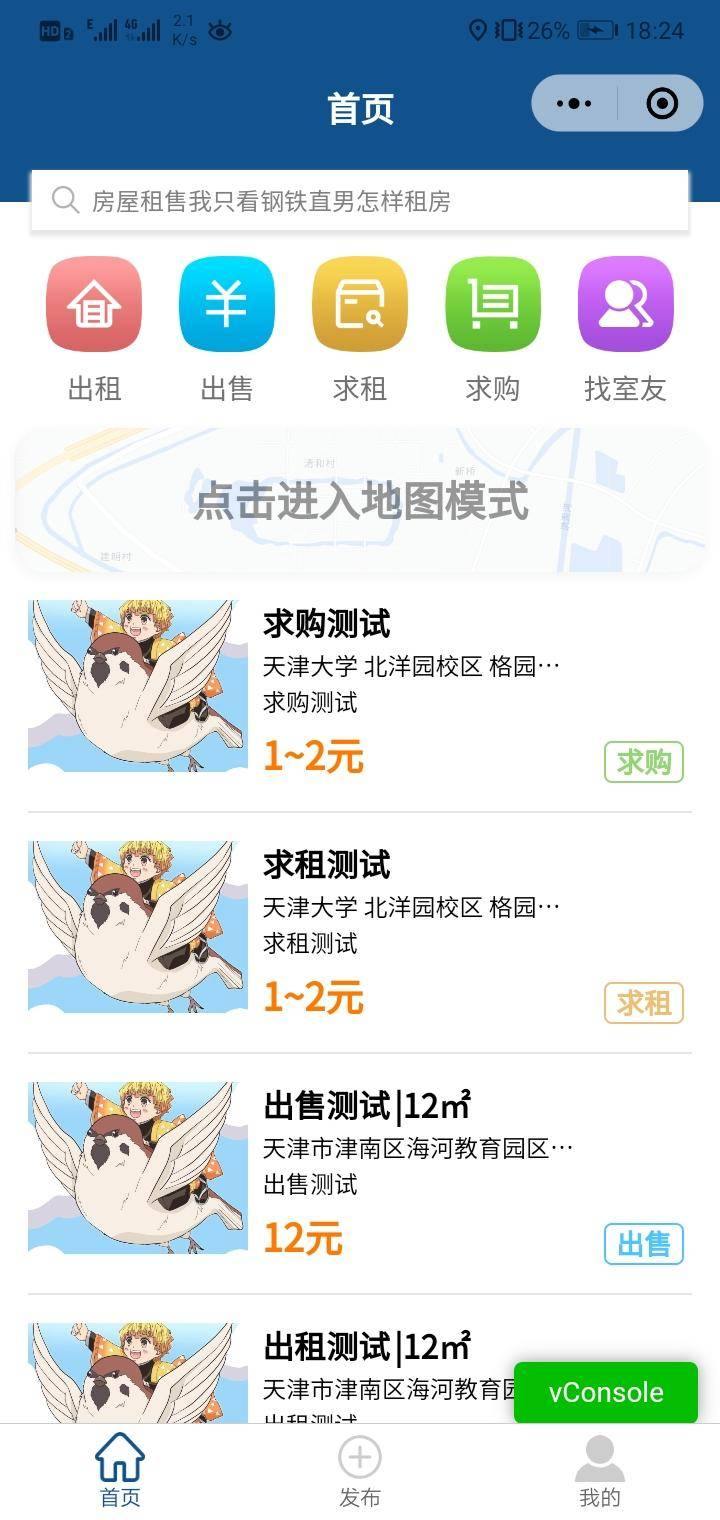
\includegraphics[width=4cm,height=8cm]{test/image/test33.png}
    \caption{测试结果}
    \end{minipage}
    \end{figure} 

   \section{发布找室友帖子功能测试}

实现用例10:发布找室友信息

功能描述:用户可以发布找室友信息

用户操作:在”发布“界面点击”我要找室友“按钮,进入信息填写界面,填写后点击发布

预期结果:页面跳转到”首页“

测试结果:通过
\newpage 
\begin{figure}[htbp]
    \centering
    \begin{minipage}[t]{0.48\textwidth}
    \centering
    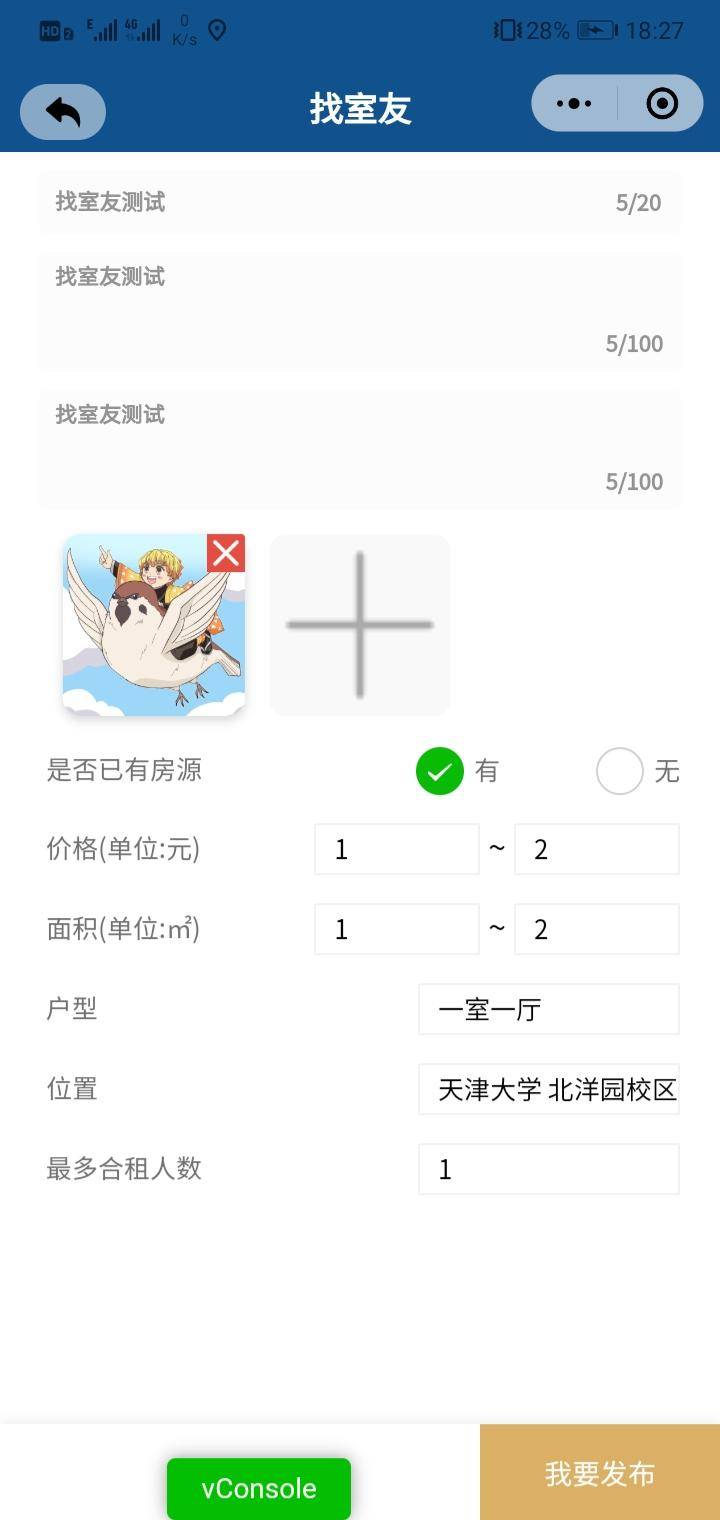
\includegraphics[width=4cm,height=8cm]{test/image/test34.png} 
 
   \caption{发布找室友信息} 
    \end{minipage}
    \begin{minipage}[t]{0.48\textwidth}
    \centering
    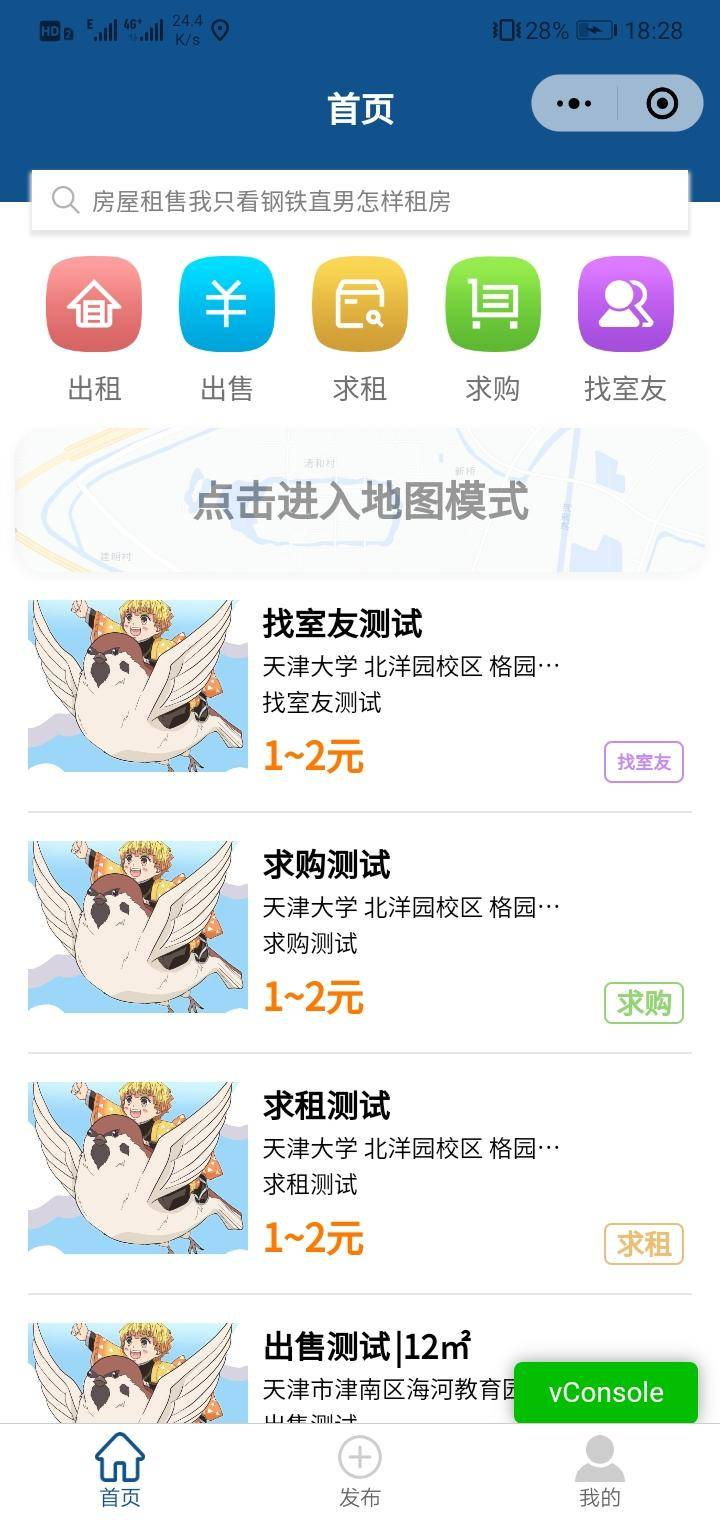
\includegraphics[width=4cm,height=8cm]{test/image/test35.png}
    \caption{测试结果}
    \end{minipage}
    \end{figure}


   \section{管理帖子功能测试}

   实现用例6,8,11,13,15:管理出售房屋信息,管理出租房屋信息,管理找室友信息,管理求租信息,管理求购信息

   功能描述:用户可以管理自己发布的出售、出租、找室友、求租、求购帖子
   
   用户操作:用户点击自己发出的帖子,进入详情页后可以删除该帖子
   
   预期结果:页面跳转到”首页“
   
   测试结果:通过
   
   \begin{figure}[htbp]
       \centering
       \begin{minipage}[t]{0.48\textwidth}
       \centering
       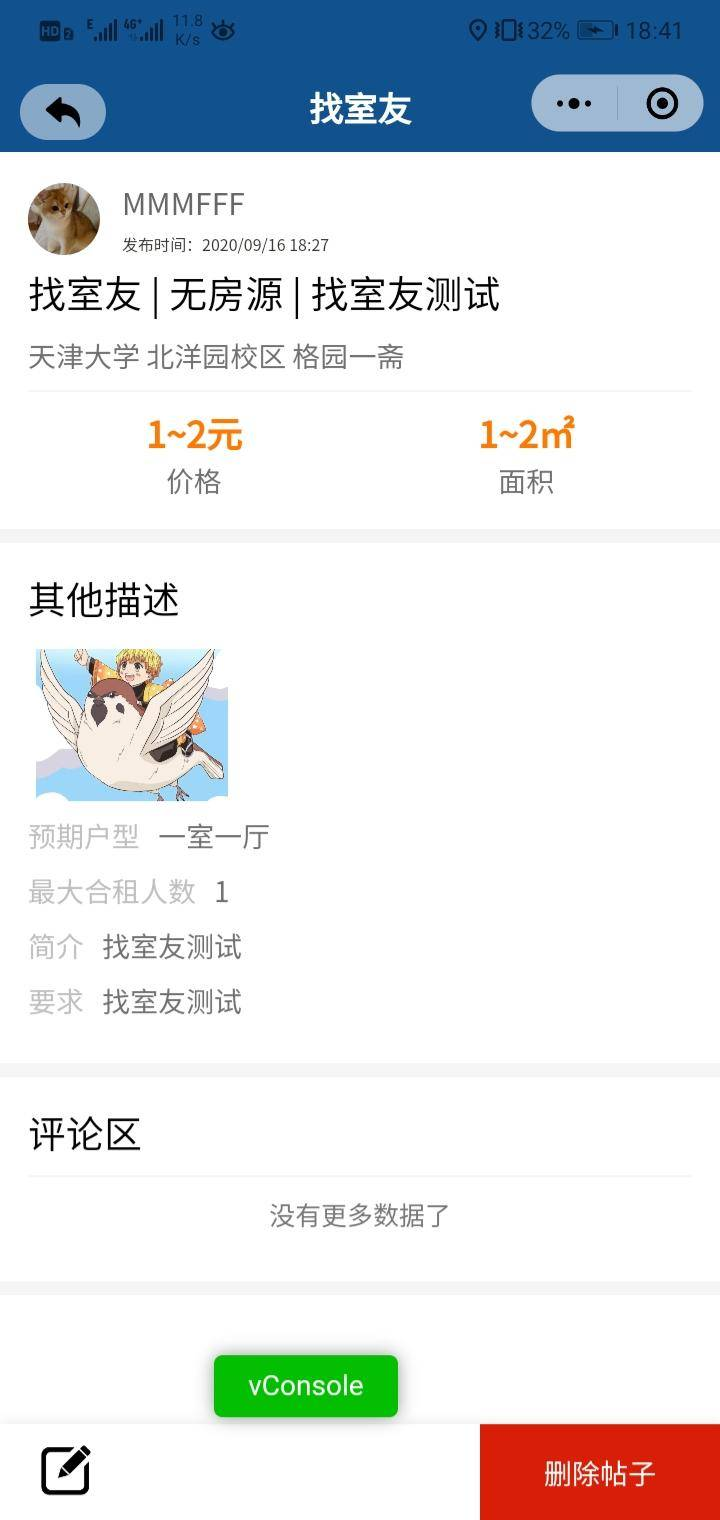
\includegraphics[width=4cm,height=8cm]{test/image/test36.png} 
    
      \caption{管理帖子} 
       \end{minipage}
       \begin{minipage}[t]{0.48\textwidth}
       \centering
       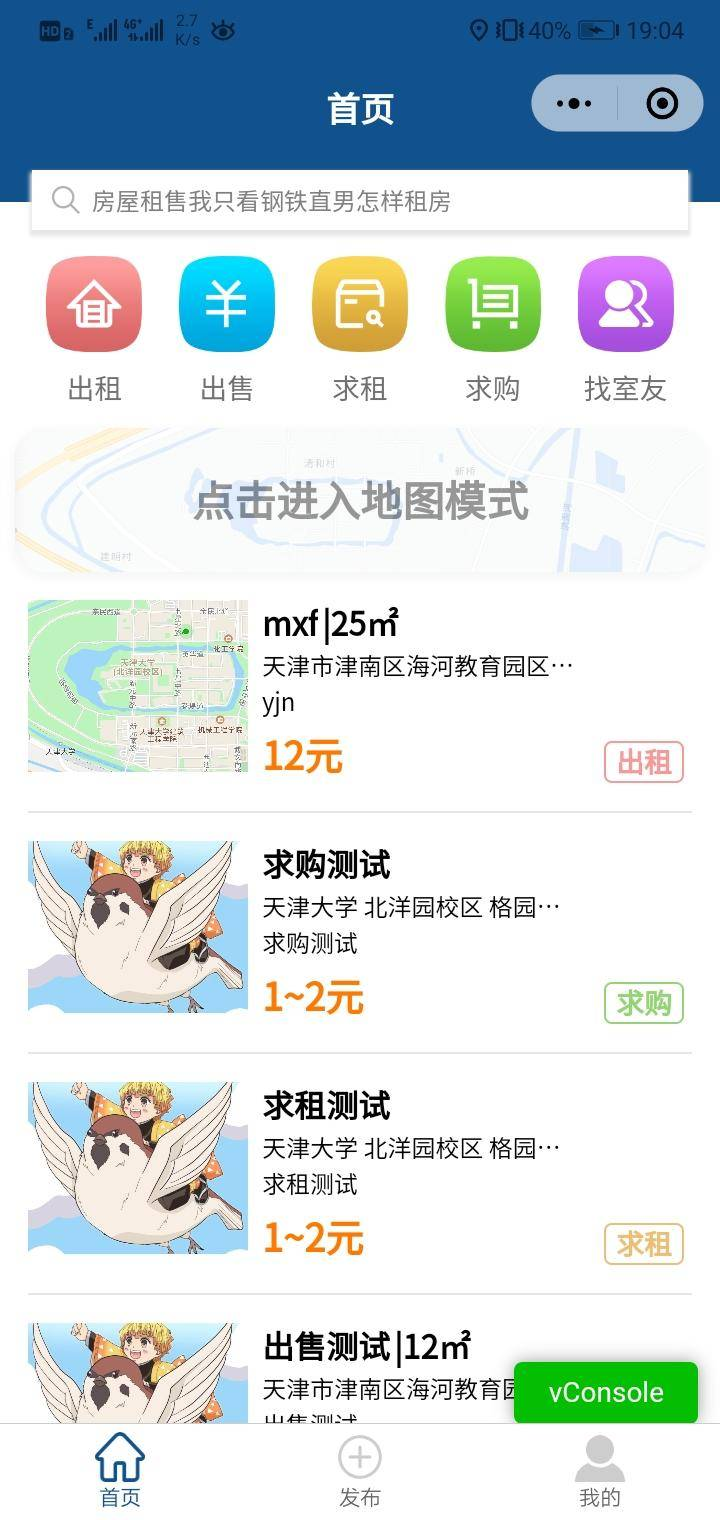
\includegraphics[width=4cm,height=8cm]{test/image/test37.png}
       \caption{结果}
       \end{minipage}
       \end{figure}
      \newpage 

   \section{评论功能测试}

   实现用例2:评论留言功能

   功能描述:用户可以在他人的帖子下发表评论,也可回复他人评论
   
   用户操作:用户点击详情页中的写评论图标,填写评论点击确定
   
   预期结果:帖子下方出现发表的评论
   
   测试结果:通过
   
   \begin{figure}[htbp]
       \centering
       \begin{minipage}[t]{0.48\textwidth}
       \centering
       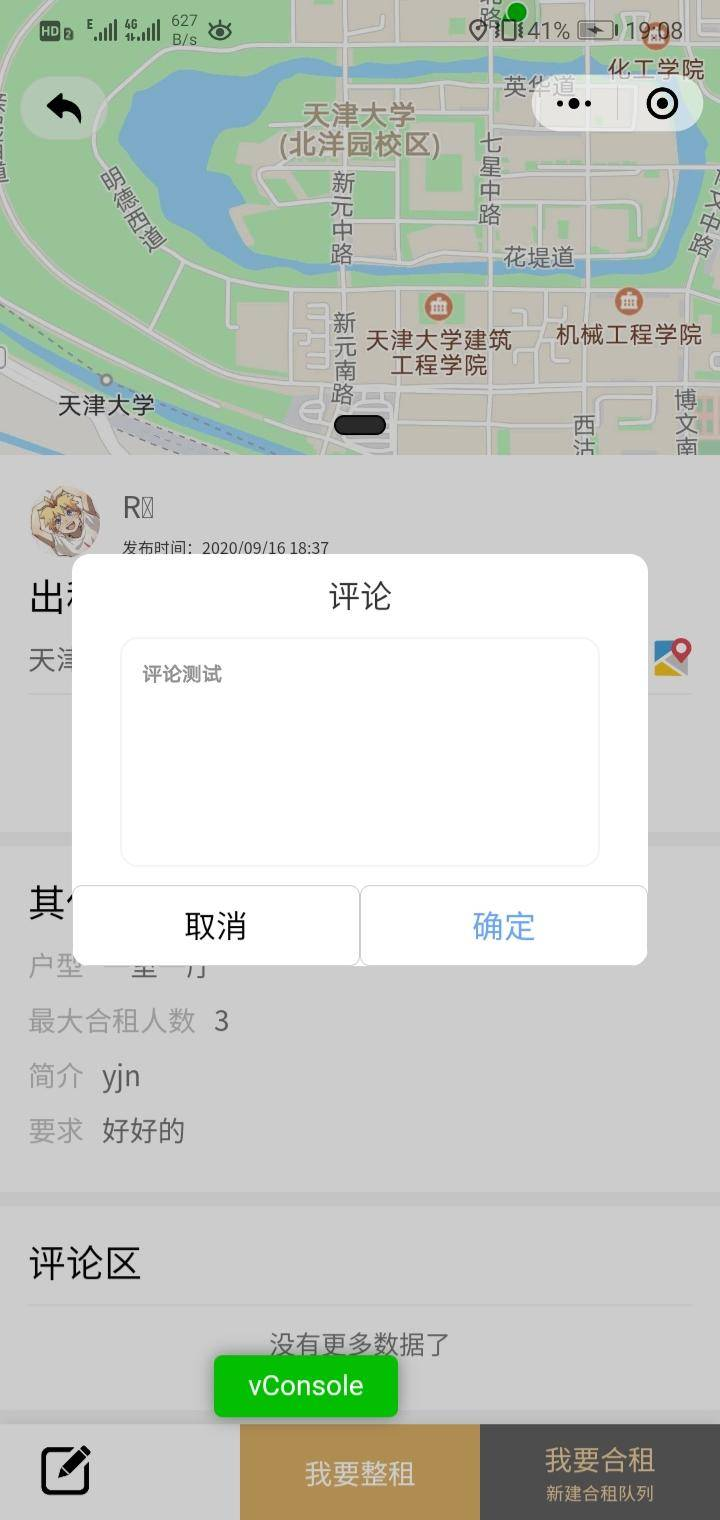
\includegraphics[width=4cm,height=8cm]{test/image/test38.png} 
    
      \caption{评论} 
       \end{minipage}
       \begin{minipage}[t]{0.48\textwidth}
        \centering
        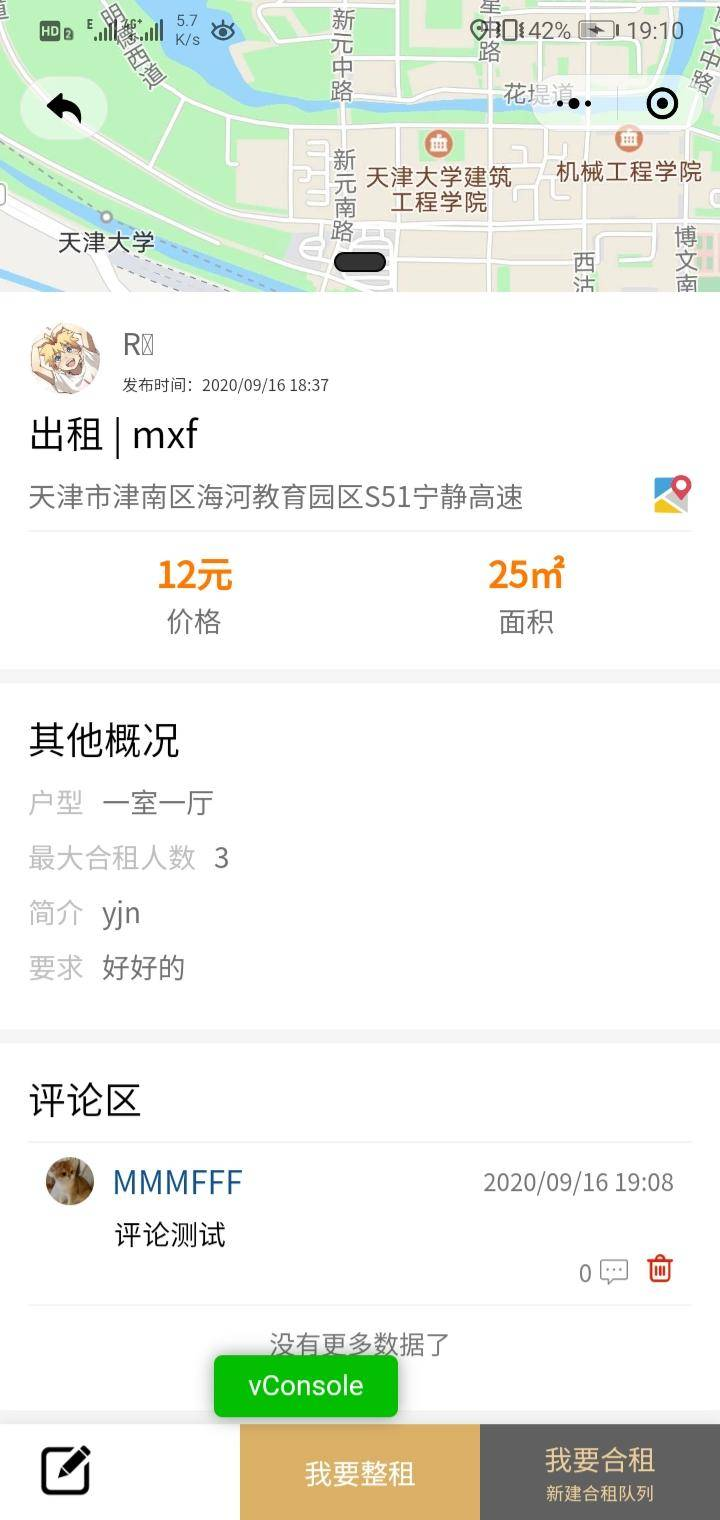
\includegraphics[width=4cm,height=8cm]{test/image/test39.png} 
     
       \caption{结果} 
         \end{minipage}
       \end{figure}
 
   \section{创建合租队列功能测试}
 
   功能描述:用户可以在他人的出租帖子下创建合租队列
   
   用户操作:用户点击详情页中的我要合租按钮 点击确定
   
   预期结果:帖子下方出现用户的合租队列
   
   测试结果:通过
   \newpage 
   \begin{figure}[htbp]
       \centering
       \begin{minipage}[t]{0.48\textwidth}
       \centering
       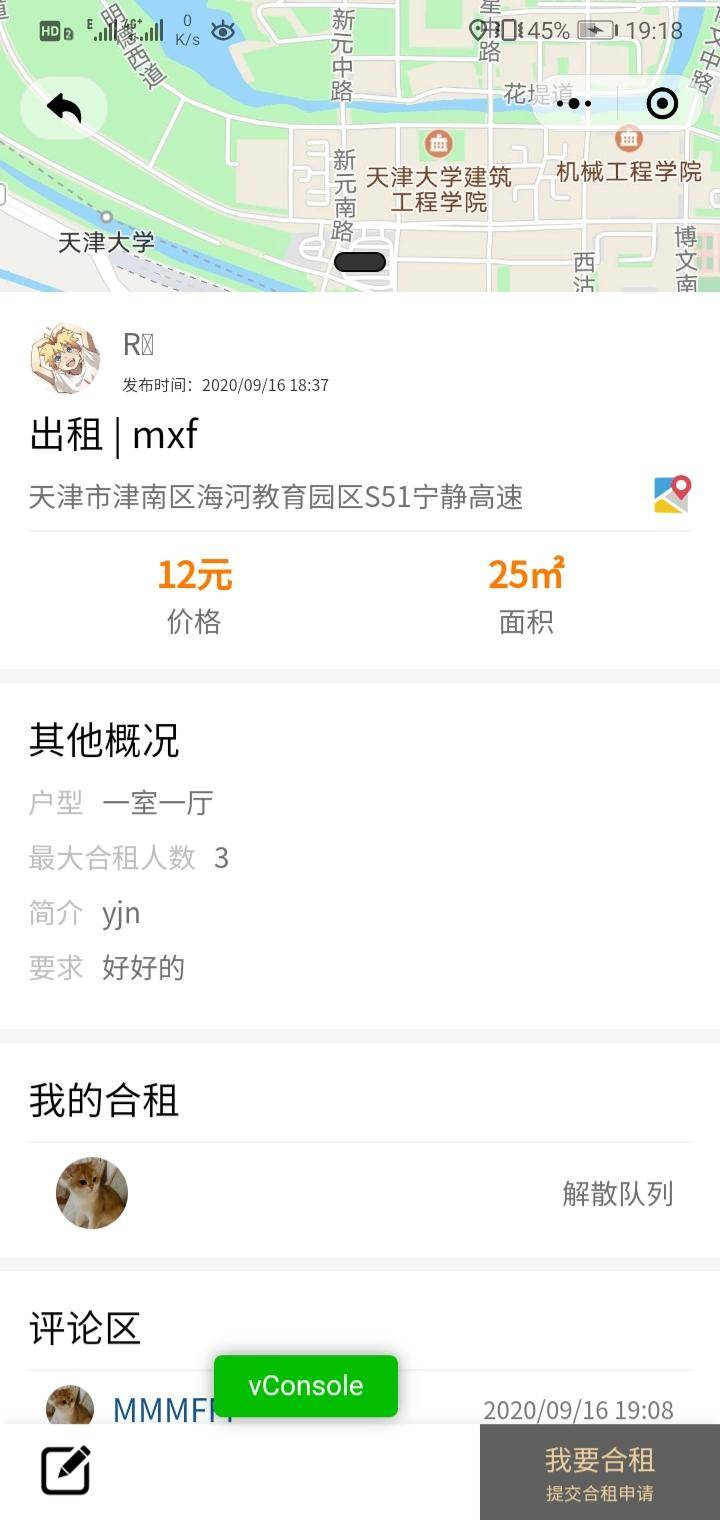
\includegraphics[width=4cm,height=8cm]{test/image/test40.png} 
    
      \caption{创建合租队列功能测试} 
       \end{minipage}
        
       \end{figure}
 

   \section{加入合租队列功能测试}
   功能描述:用户可以加入他人的合租队列
   
   用户操作:用户点击详情页中合租队列后的加入按钮
   
   预期结果:帖子详情页出现我的队列
   
   测试结果:通过
   
   \begin{figure}[htbp]
       \centering
       \begin{minipage}[t]{0.48\textwidth}
       \centering
       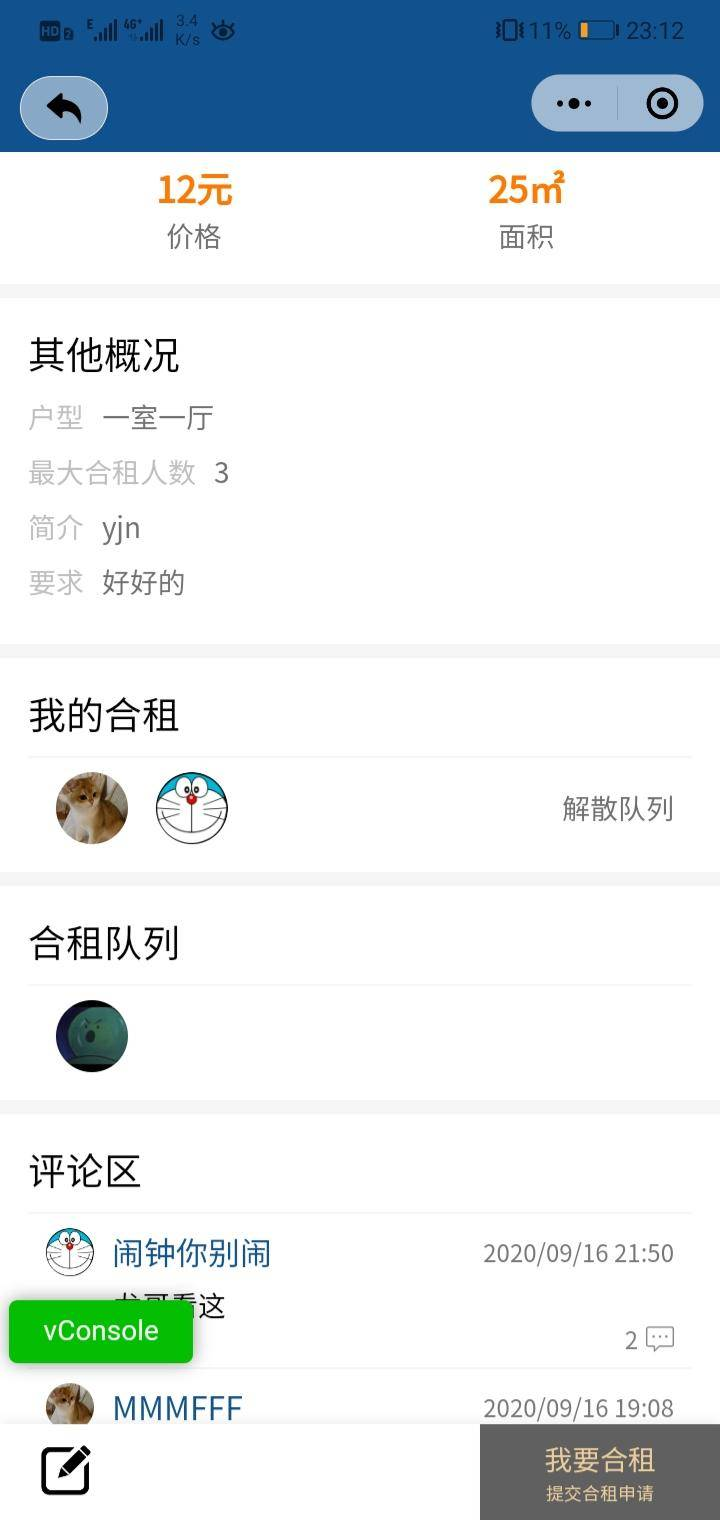
\includegraphics[width=4cm,height=8cm]{test/image/test41.png} 
    
      \caption{加入合租列队功能测试} 
    \end{minipage}
       \end{figure}
      \newpage 

   \section{删除合租队列功能测试}
 
   功能描述:合租队伍 发起者可以解散合租队伍
   
   用户操作:用户点击自己队伍旁的解散队伍按钮,并点击确定
   
   预期结果:详情页中自己的合租队伍被删除   
   
   测试结果:通过
   
   \begin{figure}[htbp]
       \centering
       \begin{minipage}[t]{0.48\textwidth}
       \centering
       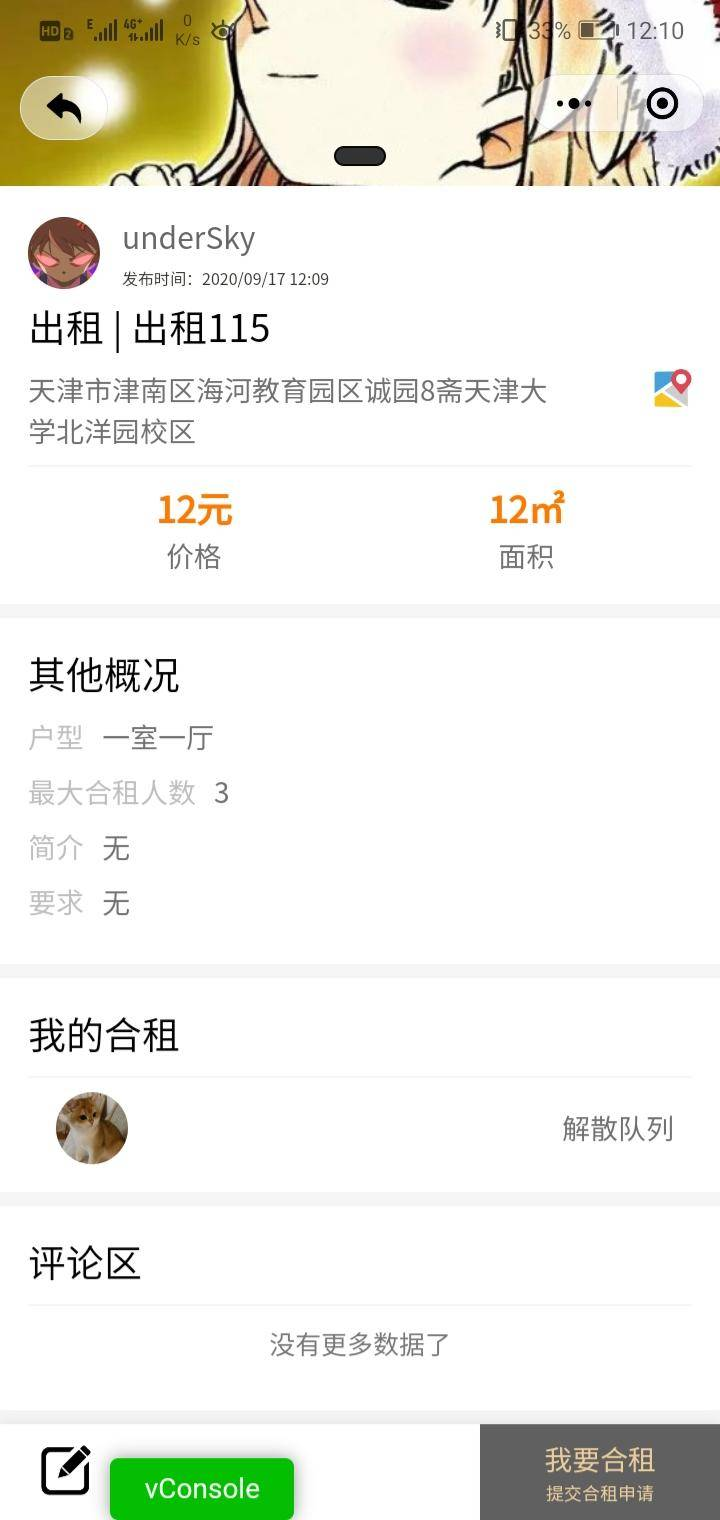
\includegraphics[width=4cm,height=8cm]{test/image/test42.png} 
    
      \caption{删除合租队列功能测试} 
       \end{minipage}
       \begin{minipage}[t]{0.48\textwidth}
       \centering
       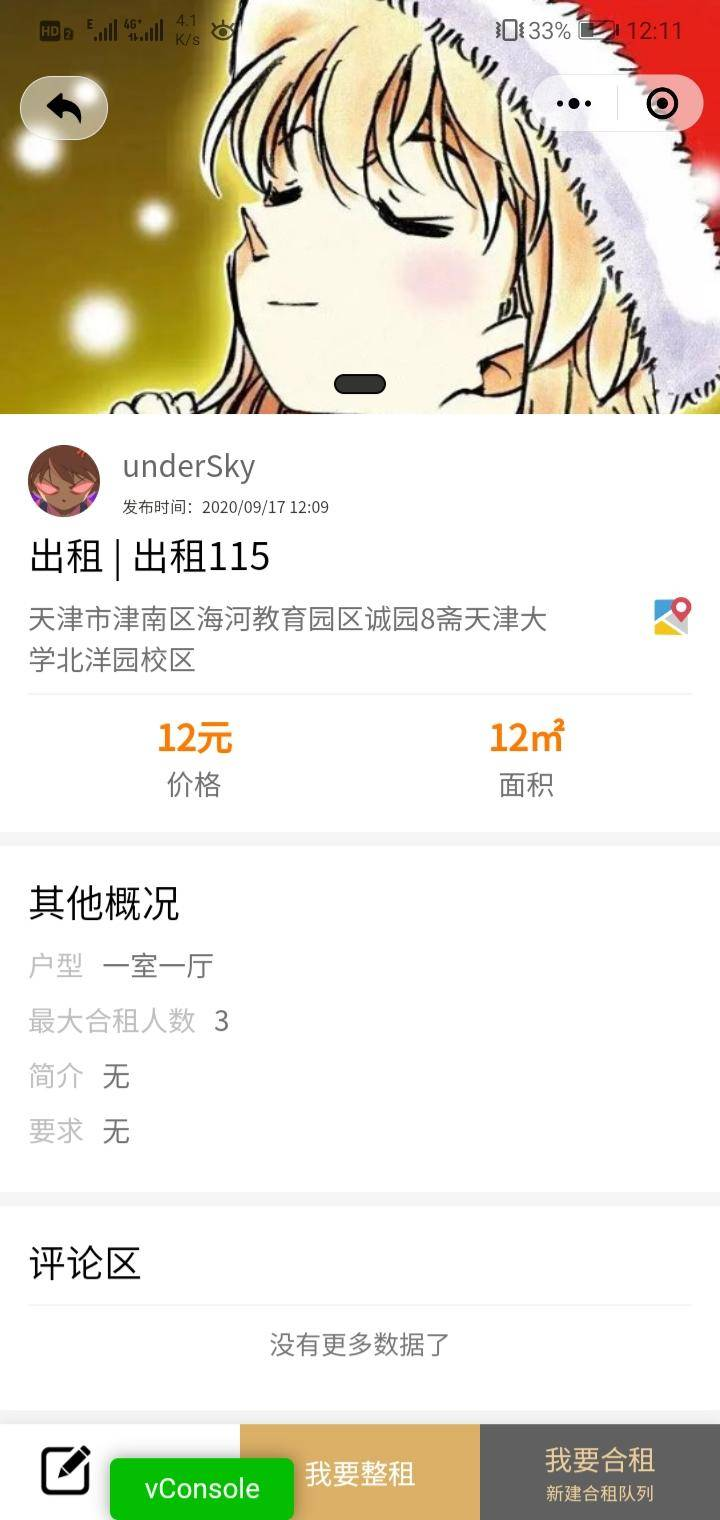
\includegraphics[width=4cm,height=8cm]{test/image/test43.png}
       \caption{测试结果}
       \end{minipage}
       \end{figure}
   
   \section{同意帖子功能测试}
   功能描述:1.用户可以以合租队长身份或个人身份向房住发出租房申请2.用户可以以个人身份向帖子主发出租房/购房/提供房源/找室友/的请求
   
   用户操作:用户以队长身份点击”发出申请“按钮或以个人身份点击我要“整租”
   
   预期结果:帖子主可以在帖子中看到他人的申请
   
   测试结果:通过
   \newpage 
   \begin{figure}[htbp]
       \centering
       \begin{minipage}[t]{0.48\textwidth}
       \centering
       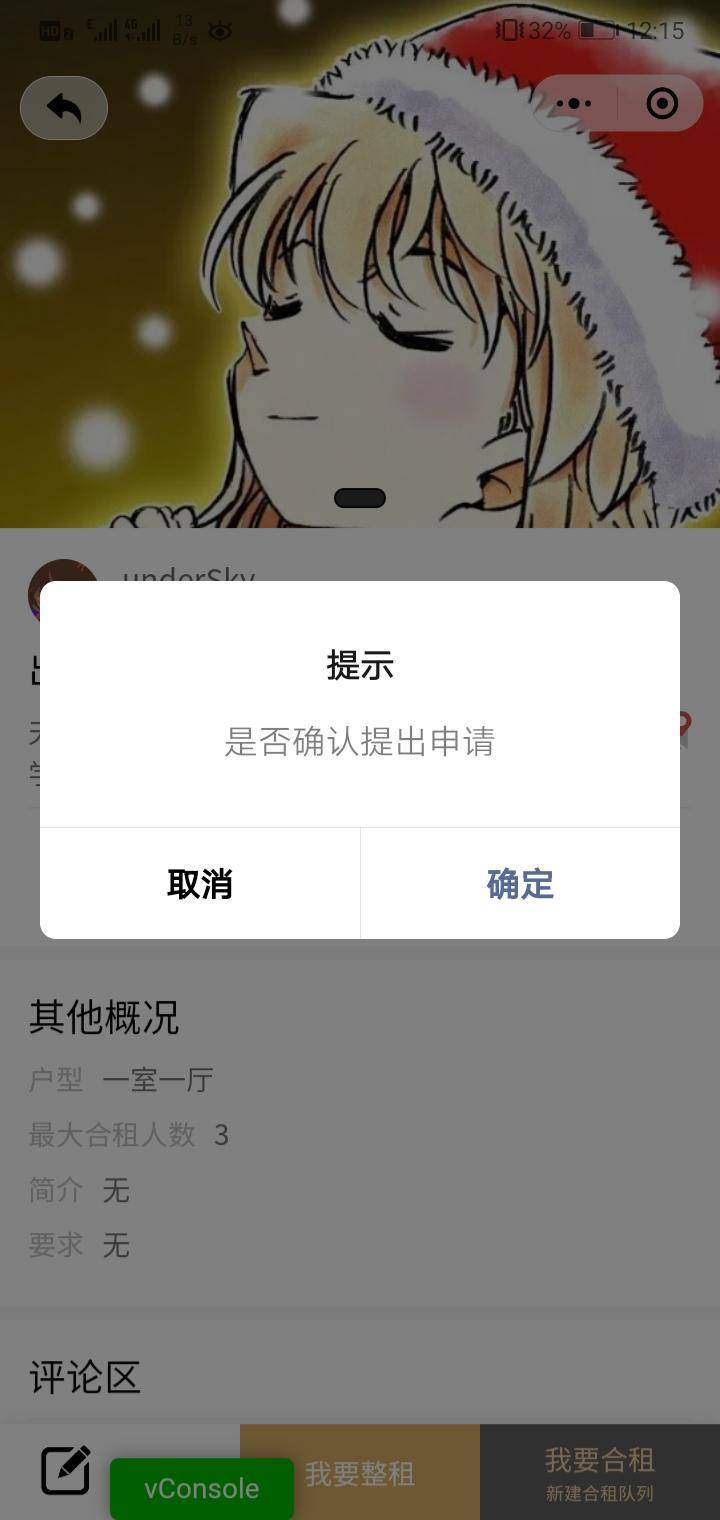
\includegraphics[width=4cm,height=8cm]{test/image/test44.png} 
    
      \caption{合租申请} 
    \end{minipage}
      \begin{minipage}[t]{0.48\textwidth}
        \centering
        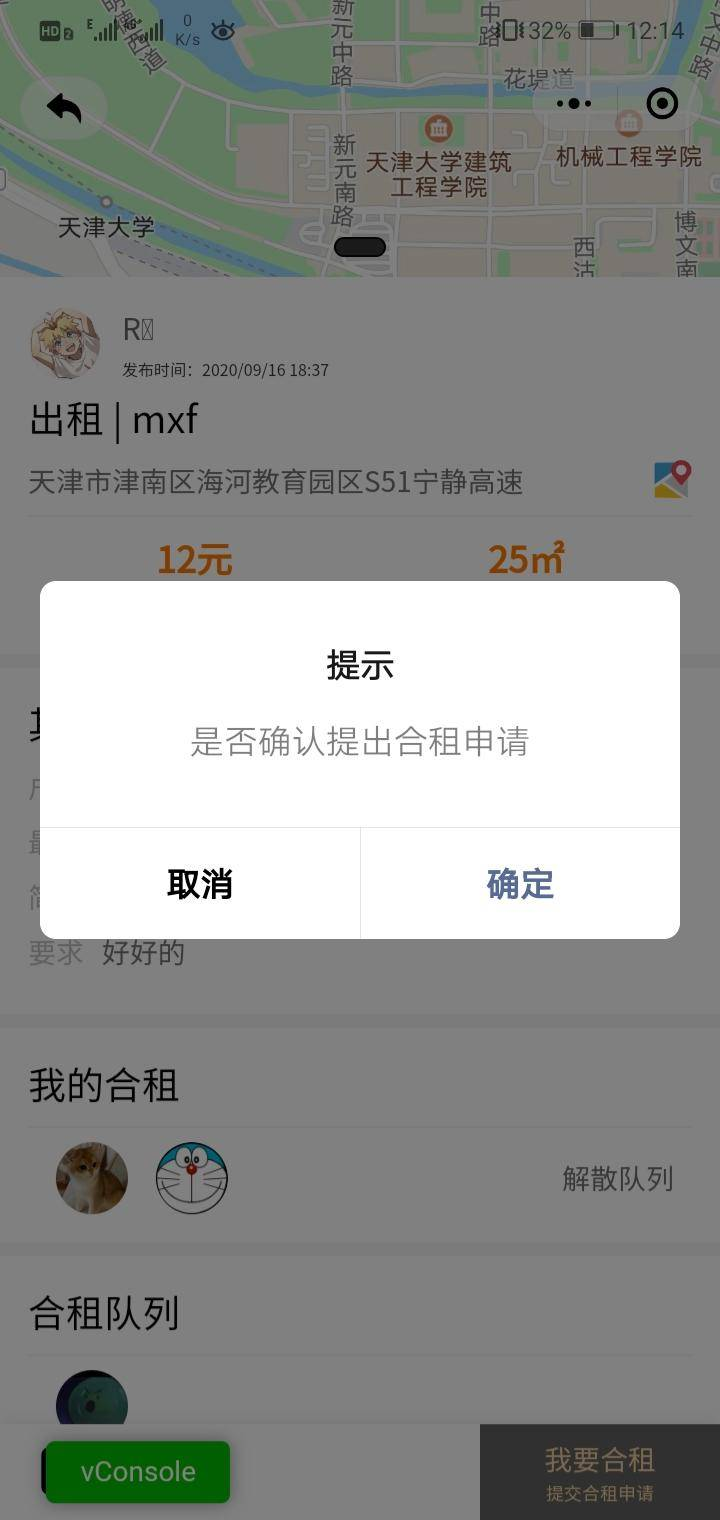
\includegraphics[width=4cm,height=8cm]{test/image/test45.png} 
     
       \caption{整租申请} 
        \end{minipage}
       \end{figure}
    
   \section{同意申请功能测试}
   完成用例4:接单

   功能描述:帖子主可以同意他人的申请
   
   用户操作:用户在帖子详情页可以点击申请队列处的同意申请
   
   预期结果:同意后帖子被转至已完成
   
   测试结果:通过
   
   \begin{figure}[htbp]
       \centering
       \begin{minipage}[t]{0.48\textwidth}
       \centering
       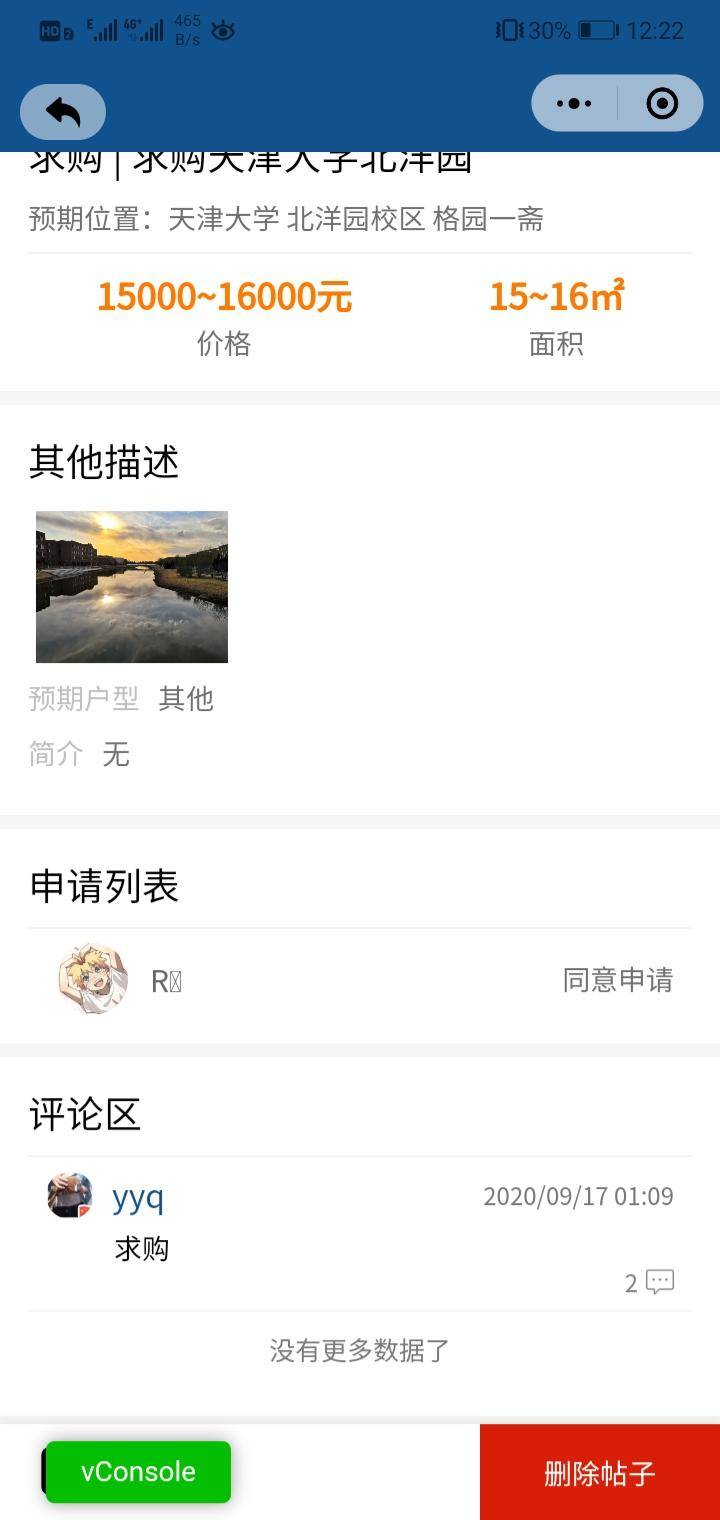
\includegraphics[width=4cm,height=8cm]{test/image/test46.png} 
    
      \caption{申请功能测试} 
             \end{minipage}
       \end{figure}
      \newpage 
   \section{查看未完成帖子功能测试}
 
   功能描述:用户可以查看自己发出请求和发布的未完成的帖子
   
   用户操作:用户在“我的”页面下点击”未完成订单“按钮
   
   预期结果:页面跳转到”未完成订单
   
   测试结果:通过
 
   \begin{figure}[htbp]
       \centering
       \begin{minipage}[t]{0.48\textwidth}
       \centering
       \includegraphics[width=4cm,height=8cm]{test/image/test47.png} 
    
      \caption{搜索结果} 
       \end{minipage}
       \begin{minipage}[t]{0.48\textwidth}
       \centering
       \includegraphics[width=4cm,height=8cm]{test/image/test48.png}
       \caption{未完成界面}
       \end{minipage}
       \end{figure}
    
   \section{查看已完成帖子功能测试}
   功能描述:用户可以查看自己发出请求和发布的已完成的帖子,
   
   用户操作:用户在“我的”页面下点击”已完成订单“按钮
   
   预期结果:页面跳转到”已完成订单“
   
   测试结果:通过
   
   \begin{figure}[htbp]
       \centering
       \begin{minipage}[t]{0.48\textwidth}
       \centering
       \includegraphics[width=4cm,height=8cm]{test/image/test49.png} 
    
      \caption{我的界面} 
       \end{minipage}
       \begin{minipage}[t]{0.48\textwidth}
        \centering
        \includegraphics[width=4cm,height=8cm]{test/image/test50.png} 
     
       \caption{已完成界面}
    \end{minipage}
       \end{figure}
      \newpage 
   \section{查看通知功能测试}
   功能描述:用户可以查看其他用户发出的与自己有关的操作的提醒
   
   用户操作:用户点击“我的”可查看消息队列
   
   预期结果:页面跳转到”我的”页面
   
   测试结果:通过

   \begin{figure}[htbp]
       \centering
       \begin{minipage}[t]{0.48\textwidth}
       \centering
       \includegraphics[width=4cm,height=8cm]{test/image/test51.png} 
    
      \caption{通知} 
       \end{minipage}
 
       \end{figure}
       \newpage 
   \section{查看个人资料功能测试}
   完成用例18:查看用户信息

   功能描述:用户可以查看自己的个人资料
   
   用户操作:用户点击“我的”中的头像可以查看自己的个人信息
   
   预期结果:页面跳转到”个人信息”页面
   
   测试结果:通过
   
   \begin{figure}[htbp]
       \centering
       \begin{minipage}[t]{0.48\textwidth}
       \centering
       \includegraphics[width=4cm,height=8cm]{test/image/test52.png}
       \caption{个人信息界面}
       \end{minipage}
       \end{figure}
      \newpage 
   \section{修改个人资料功能测试}
   完成用例18:查看用户信息

   功能描述:用户可以修改自己的个人资料
   
   用户操作:可在个人信息界面修改个人信息
   
   预期结果:个人信息发生改变
   
   测试结果:个人简介修改,测试通过
   
   \begin{figure}[htbp]
       \centering
       \begin{minipage}[t]{0.48\textwidth}
       \centering
       \includegraphics[width=4cm,height=8cm]{test/image/test53.png} 
      \caption{个人信息界面} 
       \end{minipage}
       \begin{minipage}[t]{0.48\textwidth}
        \centering
        \includegraphics[width=4cm,height=8cm]{test/image/test55.png} 
       \caption{修改后} 
        \end{minipage}
       \end{figure}
      \newpage 

      \section{地图查看出租/出售帖子信息展示功能测试}
      完成用例1:房屋信息查询
   
      功能描述:用户可以在地图上查看出租/出售资源位置
      
      用户操作:用户点击“首页”的“点击进入地图模式”按钮
      
      预期结果:跳转到地图界面,地图上展示房屋资源
      
      测试结果:通过
      
      \begin{figure}[htbp]
          \centering
          \begin{minipage}[t]{0.48\textwidth}
          \centering
          \includegraphics[width=4cm,height=8cm]{test/image/test56.png} 
         \caption{个人信息界面} 
          \end{minipage}
          \begin{minipage}[t]{0.48\textwidth}
           \centering
           \includegraphics[width=4cm,height=8cm]{test/image/test57.png} 
          \caption{修改后} 
           \end{minipage}
          \end{figure}
         \newpage 
         \section{通过地图查看出租/出售帖子位置功能测试}
         完成用例1:房屋信息查询
      
         功能描述:用户可以在地图上查看指定出租/出售资源位置
         
         用户操作:用户点击“详情页”的“地图”按钮
         
         预期结果:跳转到地图界面,地图上展示房屋资源
         
         测试结果:通过
         
         \begin{figure}[htbp]
             \centering
             \begin{minipage}[t]{0.48\textwidth}
             \centering
             \includegraphics[width=4cm,height=8cm]{test/image/test58.png} 
            \caption{个人信息界面} 
             \end{minipage}
             \begin{minipage}[t]{0.48\textwidth}
              \centering
              \includegraphics[width=4cm,height=8cm]{test/image/test59.png} 
             \caption{修改后} 
              \end{minipage}
             \end{figure}
            \newpage                